% *created  "Fri Jun  5 12:11:18 2020" *by "Paul E. Black"
% *modified "Fri Jul  7 16:07:30 2023" *by "Paul E. Black"

\documentclass[12pt]{article}
\usepackage{amsmath}
\usepackage{amsfonts}   % if you want the fonts
\usepackage{amssymb}    % if you want extra symbols
\usepackage{graphicx}   % need for figures
\usepackage{xcolor}
\usepackage{bm}
\usepackage{secdot}		
\usepackage{mathptmx}
\usepackage{float}
\usepackage[utf8]{inputenc}
\usepackage{textcomp}
\usepackage[hang,flushmargin,bottom]{footmisc} % footnote format

\usepackage{titlesec}
\titleformat{\section}{\normalsize\bfseries}{\thesection.}{1em}{}	% required for heading numbering style
\titleformat*{\subsection}{\normalsize\bfseries}

\usepackage{tocloft}	% change typeset, titles, and format list of appendices/figures/tables
\renewcommand{\cftdot}{}	
\renewcommand{\contentsname}{Table of Contents}
\renewcommand{\cftpartleader}{\cftdotfill{\cftdotsep}} % for parts
\renewcommand{\cftsecleader}{\cftdotfill{\cftdotsep}}
\renewcommand\cftbeforesecskip{\setlength{4pt}{}}
\addtolength{\cftfignumwidth}{1em}
\renewcommand{\cftfigpresnum}{\figurename\ }
\addtolength{\cfttabnumwidth}{1em}
\renewcommand{\cfttabpresnum}{\tablename\ }
\setlength{\cfttabindent}{0in}    %% adjust as you like
\setlength{\cftfigindent}{0in} 

\setcounter{tocdepth}{2} % only show down to subsections

\usepackage{enumitem}         % to control spacing between bullets/numbered lists
%\setlist{nosep} % no space between list items or around lists

\usepackage[numbers,sort&compress]{natbib} % format bibliography 
\renewcommand{\bibsection}{}
\setlength{\bibsep}{0.0pt}

% hyphenate URLs in more places (must precede hyperref)
\usepackage[hyphens,obeyspaces]{url}
\usepackage[hidelinks]{hyperref}
\hypersetup{
	colorlinks = true,
urlcolor ={blue},
citecolor = {.},
linkcolor = {.},
anchorcolor = {.},
filecolor = {.},
menucolor = {.},
runcolor = {.}
pdftitle={},
pdfsubject={},
pdfauthor={},
pdfkeywords={}
}
\urlstyle{same}

\usepackage{epstopdf} % converting EPS figure files to PDF

\usepackage{fancyhdr, lastpage}	% formatting document, calculating number of pages, formatting headers
\setlength{\topmargin}{-0.5in}
\setlength{\headheight}{39pt}
\setlength{\oddsidemargin}{0.25in}
\setlength{\evensidemargin}{0.25in}
\setlength{\textwidth}{6.0in}
\setlength{\textheight}{8.5in}

\usepackage{caption} % required for Figure labels
\captionsetup{font=small,labelfont=bf,figurename=Fig.,labelsep=period,justification=raggedright} 

% put a light gray ``DRAFT'' diagonally across each page
\usepackage{draftwatermark}
% datetime2 replaces datetime.
% DTMenglishshortmonthname replaces shortmonthname, but it doesn't work.
\usepackage{datetime} % for short month name, e.g. Jan, Feb, Mar, etc.
\SetWatermarkText{DRAFT \number\day\ \shortmonthname\ \the\year}
% bigger percentage is closer to white
\SetWatermarkColor[gray]{0.9}
\SetWatermarkFontSize{3cm}
\SetWatermarkAngle{55}
\SetWatermarkHorCenter{11cm}

\usepackage{xcolor} % for colored text and backgrounds

%%%%%%%%%%% !!!!!! REQUIRED - FILL OUT METADATA FOR NISTIR HERE !!!!!!!! %%%%%%%%%%%%%%
%  	Report Number - fill in Report Number sent to you (see info below)
%   DOI Statement - fill in DOI sent to you 
%   Month Year - fill in Month and Year of Publication
%%%%%%%%%%%%%%%%%%%%%%%%%%%%%%%%%%%%%%%%%%%%%%%%%%%%%%%%%%%%%%%%%%%%%%%%%%%%%%%%%%%%%%
\newcommand{\pubnumber}{XXXX}
\newcommand{\DOI}{https://doi.org/10.6028/NIST.IR.XXXX}
\newcommand{\monthyear}{March 2023}
\newcommand{\paperTitle}{Vulnerability Test Suite Generator (VTSG) Version 3}

%%%%%%%%%%%%%%%%%%%%%%%%%%%%%%%%%%%%%%%%%%%%%%%%%%%%%%%%%%%%%%%%%%%%
%   	BEGIN DOCUMENT 
%%%%%%%%%%%%%%%%%%%%%%%%%%%%%%%%%%%%%%%%%%%%%%%%%%%%%%%%%%%%%%%%%%%%

% correct bad hyphenation here
\hyphenation{e-qua-tion}

% list of commands for horizontal spacing---and there are a LOT of them---and
% examples of each one
% https://tex.stackexchange.com/questions/74353/what-commands-are-there-for-horizontal-spacing

% to wrap paragraph in table cells
\usepackage{makecell}

% typeset C#
% According to the ECMA-334 C# Language Specification, 5th
% Edition, Sec. 5, Acronyms and abbreviations, ``The name 
% C# is written as the LATIN CAPITAL LETTER C (U+0043) followed 
% by the NUMBER SIGN # (U+0023).'' \cite{ECMA-CSharp2017}
% https://www.ecma-international.org/publications/standards/Ecma-334.htm
% Dec 2017, Accessed: 12 June 2020
\newcommand{\CSharp}{C{\fontseries{b}\selectfont\#}}
% another possibility is C\nolinebreak\#\

% zero-width space, so "--" does not become en dash
\newcommand{\zws}{\hspace{0pt}}

\begin{document}
	\urlstyle{rm} % Format style of \url   

%%%%%%%%%%%%%%%%%%%%%%%%%%%%%%%%%%%%%%%%%%%%%%%%%%%%%%%%%%%%%%%%%%%%
%   Cover Page is REQUIRED and must contain the information 
%	displayed here, at a minimum. Additional artwork may be included 
%	(e.g., official project/conference logo, etc.).
%	Pub Number automated based on metadata
%%%%%%%%%%%%%%%%%%%%%%%%%%%%%%%%%%%%%%%%%%%%%%%%%%%%%%%%%%%%%%%%%%%%
\begin{titlepage}
\begin{flushright}
%%%%%%%%%%%%%%%%%%%%%%%%%%%%%%%%%%%%%%%%%%%%%%%%%%%%%%%%%%%%%%%%%%%%
% 	Automated based on metadata - delete if not applicable
%%%%%%%%%%%%%%%%%%%%%%%%%%%%%%%%%%%%%%%%%%%%%%%%%%%%%%%%%%%%%%%%%%%%
\LARGE{\textbf{NISTIR \pubnumber}}\\
\vfill
%%%%%%%%%%%%%%%%%%%%%%%%%%%%%%%%%%%%%%%%%%%%%%%%%%%%%%%%%%%%%%%%%%%%
%	Title 
%%%%%%%%%%%%%%%%%%%%%%%%%%%%%%%%%%%%%%%%%%%%%%%%%%%%%%%%%%%%%%%%%%%%
\Huge{\textbf{\paperTitle}}\\
    \vfill
%%%%%%%%%%%%%%%%%%%%%%%%%%%%%%%%%%%%%%%%%%%%%%%%%%%%%%%%%%%%%%%%%%%%
%	Authors - add complete list of authors, affiliations will be 
%   added on title page
%%%%%%%%%%%%%%%%%%%%%%%%%%%%%%%%%%%%%%%%%%%%%%%%%%%%%%%%%%%%%%%%%%%%
    \large Paul E. Black \\
    \large William Mentzer\\
    \large Elizabeth Fong \\
    \large Bertrand Stivalet
\vfill
%%%%%%%%%%%%%%%%%%%%%%%%%%%%%%%%%%%%%%%%%%%%%%%%%%%%%%%%%%%%%%%%%%%%
%	The DOI is automated based on metadata.	
%%%%%%%%%%%%%%%%%%%%%%%%%%%%%%%%%%%%%%%%%%%%%%%%%%%%%%%%%%%%%%%%%%%%
\normalsize This publication is available free of charge from:\\
\DOI\\
\vfill
%%%%%%%%%%%%%%%%%%%%%%%%%%%%%%%%%%%%%%%%%%%%%%%%%%%%%%%%%%%%%%%%%%%%
%	NIST LOGO - keep as-is
%%%%%%%%%%%%%%%%%%%%%%%%%%%%%%%%%%%%%%%%%%%%%%%%%%%%%%%%%%%%%%%%%%%%


\includegraphics[width=0.3\linewidth]{NIST-logo.eps}\\ 
 
  
\end{flushright}
\end{titlepage}
\begin{titlepage}
%%%%%%%%%%%%%%%%%%%%%%%%%%%%%%%%%%%%%%%%%%%%%%%%%%%%%%%%%%%%%%%%%%%%
%	Title Page is REQUIRED
%%%%%%%%%%%%%%%%%%%%%%%%%%%%%%%%%%%%%%%%%%%%%%%%%%%%%%%%%%%%%%%%%%%%
\begin{flushright}
%%%%%%%%%%%%%%%%%%%%%%%%%%%%%%%%%%%%%%%%%%%%%%%%%%%%%%%%%%%%%%%%%%%%
%   Publication Series & Number - automated
%%%%%%%%%%%%%%%%%%%%%%%%%%%%%%%%%%%%%%%%%%%%%%%%%%%%%%%%%%%%%%%%%%%%
\LARGE{\textbf{NISTIR \pubnumber}}\\
\vfill 
%%%%%%%%%%%%%%%%%%%%%%%%%%%%%%%%%%%%%%%%%%%%%%%%%%%%%%%%%%%%%%%%%%%%
%	Title 
%%%%%%%%%%%%%%%%%%%%%%%%%%%%%%%%%%%%%%%%%%%%%%%%%%%%%%%%%%%%%%%%%%%%
\Huge{\textbf{\paperTitle}}\\
    \vfill
%%%%%%%%%%%%%%%%%%%%%%%%%%%%%%%%%%%%%%%%%%%%%%%%%%%%%%%%%%%%%%%%%%%%
%	Author Order and Grouping. Always identify the primary author/creator first
% (s/he does not have to be a NIST author). For publications with multiple authors,
% group authors by their organizational affiliation. The organizational groupings and
% the names within each grouping should generally be ordered by decreasing level of
% contribution.
%	For non-NIST authors, list their city and state below their organization name.
%	For NIST authors, include the Division and Laboratory names (but do not
% include their city and state).
%%%%%%%%%%%%%%%%%%%%%%%%%%%%%%%%%%%%%%%%%%%%%%%%%%%%%%%%%%%%%%%%%%%%
    \normalsize 
    Paul E. Black\\
     \textit{Software and Systems Division}\\
     \textit{Information Technology Laboratory}\\
     \vspace{12pt}
    William Mentzer\\
     \textit{California State University}\\
     \textit{San Bernardino, California}\\
     \vspace{12pt}
    Elizabeth Fong \\
     \textit{affiliation}\\
     \textit{location}\\
     \vspace{12pt}
    Bertrand Stivalet \\
     \textit{affiliation}\\
     \textit{location}
\vfill
%%%%%%%%%%%%%%%%%%%%%%%%%%%%%%%%%%%%%%%%%%%%%%%%%%%%%%%%%%%%%%%%%%%%
%   DOI Statement - automated
%%%%%%%%%%%%%%%%%%%%%%%%%%%%%%%%%%%%%%%%%%%%%%%%%%%%%%%%%%%%%%%%%%%%
\normalsize This publication is available free of charge from:\\
\DOI\\
\vfill
%%%%%%%%%%%%%%%%%%%%%%%%%%%%%%%%%%%%%%%%%%%%%%%%%%%%%%%%%%%%%%%%%%%%
%   Date - Month and Year - automated
%%%%%%%%%%%%%%%%%%%%%%%%%%%%%%%%%%%%%%%%%%%%%%%%%%%%%%%%%%%%%%%%%%%%
\normalsize \monthyear
\vfill
%%%%%%%%%%%%%%%%%%%%%%%%%%%%%%%%%%%%%%%%%%%%%%%%%%%%%%%%%%%%%%%%%%%%
%  Department of Commerce LOGO - leave as-is
%%%%%%%%%%%%%%%%%%%%%%%%%%%%%%%%%%%%%%%%%%%%%%%%%%%%%%%%%%%%%%%%%%%%	


\includegraphics[width=0.18\linewidth]{DoC-logo.eps}\\ 
 \vfill
%%%%%%%%%%%%%%%%%%%%%%%%%%%%%%%%%%%%%%%%%%%%%%%%%%%%%%%%%%%%%%%%%%%%
%  Department of Commerce & NIST Leadership 
%	will be updated as changes occur
%%%%%%%%%%%%%%%%%%%%%%%%%%%%%%%%%%%%%%%%%%%%%%%%%%%%%%%%%%%%%%%%%%%%
\footnotesize U.S. Department of Commerce\\ 
\textit{Wilbur L. Ross, Jr., Secretary}\\
\vspace{10pt}
National Institute of Standards and Technology\\ 
\textit{Walter Copan, NIST Director and Undersecretary of Commerce for Standards and Technology}  
\end{flushright}
\end{titlepage}
\begin{titlepage}
%%%%%%%%%%%%%%%%%%%%%%%%%%%%%%%%%%%%%%%%%%%%%%%%%%%%%%%%%%%%%%%%%%%%
%   Disclaimer/CODEN page - required
%%%%%%%%%%%%%%%%%%%%%%%%%%%%%%%%%%%%%%%%%%%%%%%%%%%%%%%%%%%%%%%%%%%%
\begin{flushright}
\footnotesize  Certain commercial entities, equipment, or materials may be identified
in this document in order to describe an experimental procedure or concept
adequately. Such identification is not intended to imply recommendation or
endorsement by the National Institute of Standards and Technology, nor is it intended
to imply that the entities, materials, or equipment are necessarily the best
available for the purpose.\\

\vfill
%%%%%%%%%%%%%%%%%%%%%%%%%%%%%%%%%%%%%%%%%%%%%%%%%%%%%%%%%%%%%%%%%%%%
%   This section automated - do not change
%%%%%%%%%%%%%%%%%%%%%%%%%%%%%%%%%%%%%%%%%%%%%%%%%%%%%%%%%%%%%%%%%%%%
\normalsize \textbf{National Institute of Standards and Technology \\ Internal Report \pubnumber\\ 
Natl. Inst. Stand. Technol. Intern. Rep. \pubnumber, \pageref{LastPage} pages (\monthyear)} \\
\vspace{12pt}
\textbf{This publication is available free of charge from: \DOI}
\vfill
\end{flushright}
\end{titlepage}
%%%%%%%%%%%%%%%%%%%%%%%%%%%%%%%%%%%%%%%%%%%%%%%%%%%%%%%%%%%%%%%%%%%%
%   Start front matter - page number starts with "i"
%%%%%%%%%%%%%%%%%%%%%%%%%%%%%%%%%%%%%%%%%%%%%%%%%%%%%%%%%%%%%%%%%%%%
\pagenumbering{roman}

\section*{Abstract}
\normalsize
The Vulnerability Test Suite Generator (VTSG) can create vast numbers of
synthetic programs with and without specific flaws or vulnerabilities.
It was designed by the Software Assurance Metrics and Tool Evaluation (SAMATE) team
and originally implemented by students from TELECOM Nancy.
The latest version is structured to be able to generate vulnerable and nonvulnerable
synthetic programs expressing specific flaws in \emph{any} programming language.
It has libraries to generate PHP, \CSharp, and Python programs.
This document may help if you are trying to generate test cases written in 
PHP, \CSharp, or Python, adding new complexities or flaws or vulnerability, or
modifying VTSG Version 3 to generate test
cases in other programming languages.

\section*{Key words}
\normalsize Software assurance; static analyzer; test case generator; 
software vulnerabilities.

% push next part to the bottom of the page
\vfill

This document was written at the National Institute of Standards and
Technology by employees of the Federal Government in the course of
their official duties.  Pursuant to title 17 Section 105 of the United
States Code this is not subject to copyright protection and
is in the public domain.


We would appreciate acknowledgment if this document is used.

\pagebreak
%%%%%%%%%%%%%%%%%%%%%%%%%%%%%%%%%%%%%%%%%%%%%%%%%%%%%%%%%%%%%%%%%%%%
%   Table of Contents is required
% 	List of Tables & Figures required if more than 5 tables/figures
%%%%%%%%%%%%%%%%%%%%%%%%%%%%%%%%%%%%%%%%%%%%%%%%%%%%%%%%%%%%%%%%%%%%
\begin{center}
\tableofcontents
\listoftables
\listoffigures
\end{center}
\pagebreak
%%%%%%%%%%%%%%%%%%%%%%%%%%%%%%%%%%%%%%%%%%%%%%%%%%%%%%%%%%%%%%%%%%%%
%   Start body of text - page number starts with "1"
%%%%%%%%%%%%%%%%%%%%%%%%%%%%%%%%%%%%%%%%%%%%%%%%%%%%%%%%%%%%%%%%%%%%

\newpage

\section{Introduction}
\pagenumbering{arabic}

The Vulnerability Test Suite Generator (VTSG) generates collections 
of vulnerable and non-vulnerable
synthetic programs expressing specific flaws.  
The programs can be
test cases to evaluate static analyzers. 
Each test case targets one flaw. There are two types of test cases:
\begin{itemize}[nosep]
  \item cases with flawed code (unsafe), leading to a vulnerability, and
  \item safe cases with similar behavior, but without the flaws, that is, no
	vulnerability.
\end{itemize}
Exactly corresponding vulnerable and non-vulnerable
cases could, in theory, be generated in pairs. However, since each test case
is generated separately, there is no exact correspondence between 
cases.

Figure~\ref{fig:cartesian product} suggests that just three sources of input,
two ways of filtering the input, four sinks, and two ways to execute the query
already yields 3 × 2 × 4 x 2 = 48
combinations.  Multiply that by many different kinds of bugs and all flow control
complexities with various conditions, then include ``scaffolding'' such as
initializing variables, importing libraries, and declaring functions to get an
idea of the work that VTSG may save.

\begin{figure}[htbp]
  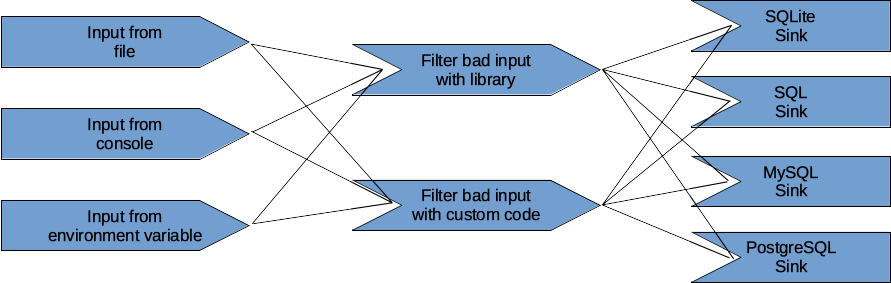
\includegraphics[width=1\linewidth]{fig_cartesian_product.png}
  \caption{Just three sources of input, two ways of filtering, four sinks, and
    two query executions yield 48 possible test cases.}
  \label{fig:cartesian product}
\end{figure}

NIST's Software Assurance Reference Dataset (SARD) has suites of paired test cases in
the Juliet test suites for C/C++ and Java, which are available as SARD test suites
108 and 109.  These and many other test suites are available at
\href{https://samate.nist.gov/SARD/testsuite.php}
     {https://samate.nist.gov/ SARD/testsuite.php}.

The generator is written in Python 3.
The VTSG git repository is at
\href{https://github.com/usnistgov/VTSG}{https://github.com/ usnistgov/VTSG}.
The list of files and the README.md file are given in App.~\ref{gitContent}.


\subsection{History} 

Originally named Vulnerability Test Suite (VTS) generator, version 1 only
generated \CSharp\ programs. VTS version 2 generated PHP
programs~\cite{StivaletFongVTSPHP2016} in addition.  Version 2 was more
customizable to generate other programming languages.
VTSG version 3 systematically maintains indentation, so also
generates Python programs.
% VTSG produces manifest files in the Static Analysis Results Interchange Format
% (SARIF) Version 2.1.0~\cite{SARIF2.1.0} format.

Readers can download the PHP and \CSharp\ test cases generated 
by earlier versions as SARD test suites 103 and 105 from
\href{https://samate.nist.gov/SARD/testsuite.php}{https://samate.nist.gov/SARD/testsuite.php}.


\subsection{Install Supporting Packages}

\noindent The following instructions are provided for users who may not have these
packages already installed on their Linux machines. Users who already have these
packages may skip this section.

\noindent To download files from Github, first install the \emph{Git} package.
Here is the command to install it:

\begin{verbatim}
    sudo apt-get install git    
\end{verbatim}

\noindent VTSG is written in Python 3, so Python 3 must be installed, too.
Here is the command to install it:

\begin{verbatim}
    sudo apt-get install python3
\end{verbatim}

\noindent To download Python source code packages, install the \emph{pip
Python} package manager.
Here is the command to install it:

\begin{verbatim}
    sudo apt-get install python-pip
\end{verbatim}

\noindent One may also have to install the \emph{pip Python 3} package manager.
Here is the command to install it:

\begin{verbatim}
    sudo apt-get install python3-pip
\end{verbatim}

\noindent Another way to install \emph{pip} is:

\begin{verbatim}
    sudo python3 -m pip install --upgrade pip
\end{verbatim}

\subsection{Install Optional Packages}

VTSG can use combinatorial testing, specifically ACTS~\cite{ACTS2013}, to select
cases instead of producing all possible cases.  The ACTS software is freely available.
To get ACTS, send email to Rick Kuhn
\href{mailto:kuhn@nist.gov}{kuhn@nist.gov}~\cite{CombinTesting}.

See App.~\ref{sec:run csharp} for instructions on how to run \CSharp\ programs.

\subsection{Install VTSG}

\noindent To copy the generic VTSG from GitHub to a local Linux machine, change to a
directory under which you want to install VTSG.

\noindent Looking at the GitHub website, one will see a green box labeled ``Code''.
See Fig.~\ref{fig:clone button}.
Click on it, then click on the ``copy'' icon to copy the web URL.

\begin{figure}[htbp]
  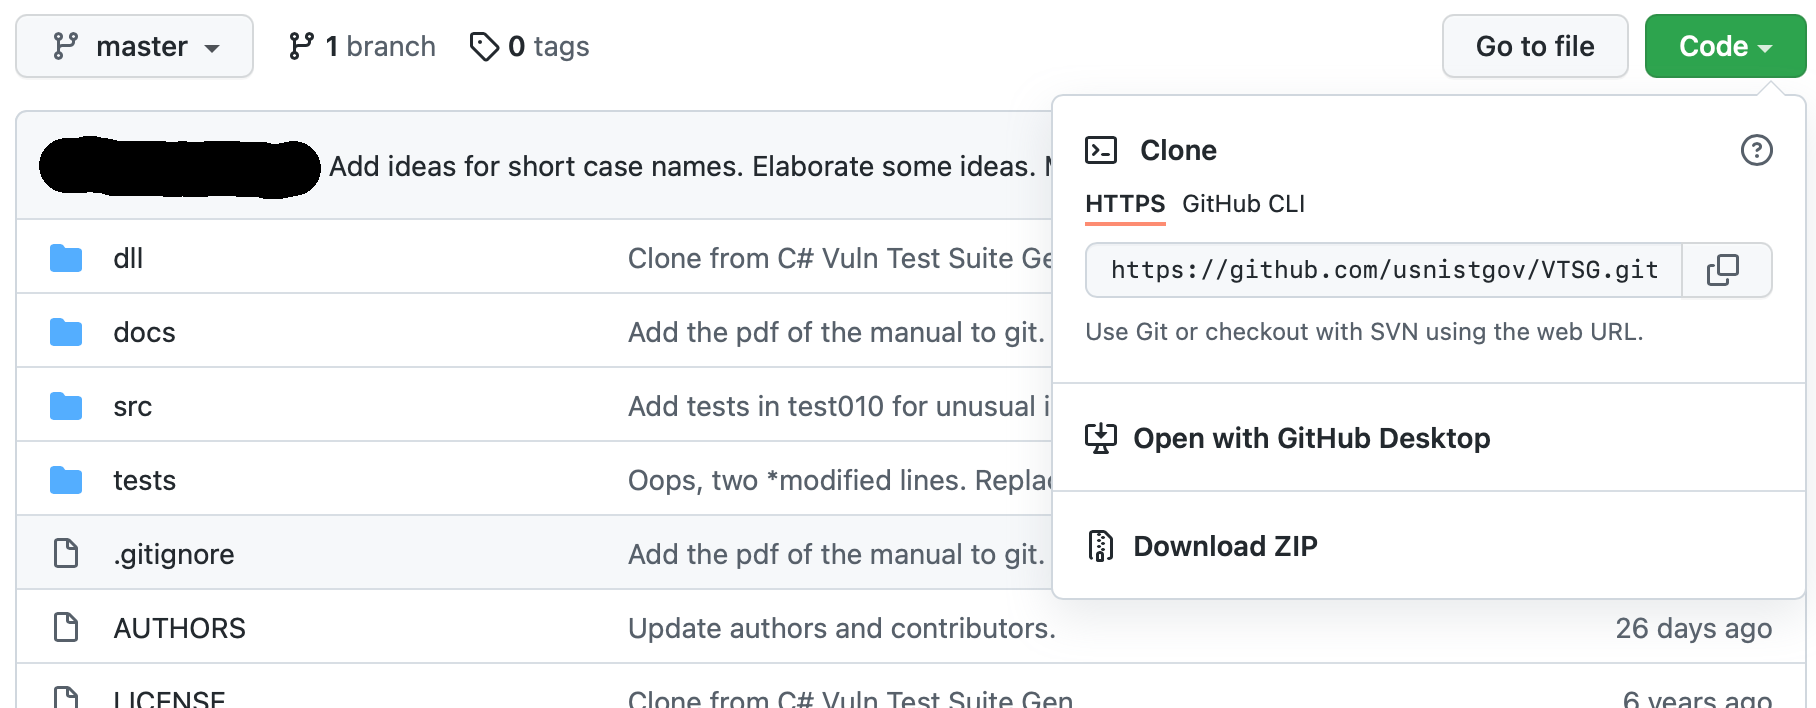
\includegraphics[width=1\linewidth]{fig_clone_tab.png}
  \caption{usnistgov/VTSG: button to clone repository.}
  \label{fig:clone button}
\end{figure}

\noindent Here is the command to copy the source code and other material to the local
directory:

\begin{verbatim}
    git clone https://github.com/usnistgov/VTSG.git
\end{verbatim}

\noindent If one types the \verb|ls| command, one will see that the \textbf{VTSG}
directory was created.

\noindent Go into that directory, using this command:

\begin{verbatim}
    cd VTSG
\end{verbatim}

\noindent To install the dependencies, use this command:

\begin{verbatim}
    pip3 install --user -r requirements.txt
\end{verbatim}


\subsection{Users}

There are two groups who will typically use VTSG. The first group comprises people
requiring test cases written in PHP, \CSharp, or Python to evaluate a static
analyzer. These users must know how to invoke VTSG with the command line interface
and retrieve the appropriate sample from the generated and categorized folders.

The second targeted audience of the VTSG comprises people wishing to generate
test cases using a programming language other than the languages currently
supported.  They must create new templates for the program
using the XML tags, execute VTSG with the command line interface,
and retrieve the samples from the generated and categorized file folders.

\subsection{Vulnerabilities Currently Encoded in VTSG Files}

Vulnerabilities are encoded in the language files, see Sec.~\ref{sec:source files}.
Some of the OWASP Top 10~\cite{OWASPTop10-2017} and
Common Weakness Enumerations (CWEs)~\cite{CWE} are encoded.
See App.~\ref{sec:CSharp language}, \ref{sec:PHP language}, and
\ref{sec:Python language} for details.


\section{Command Line Interface}
\label{sec:command line interface}

For users who wish to generate PHP, \CSharp, or Python test suites, a command line
interface
can generate all test cases or a specific group of test cases based on several
options.  For example, the user can generate vulnerable or non-vulnerable test cases
based on selected flaws or groups of flaws, for example, OWASP categories.
The user must specify the
programming language.  The invocation command looks like this:
\begin{verbatim}
$ python3 vtsg.py -l {php,cs,py} <options>
\end{verbatim}
% Overleaf complains that textcomp doesn't provide \textlangle
% and \textrangle in the font family.  So we define our own.
\newcommand{\texlangle}{$\langle$}
\newcommand{\texrangle}{$\rangle$}
where \verb|<options>| are listed in
Table~\ref{tab:command line options}.

\begin{table}[H]
\centering
\caption{Options for command line invocation}
\begin{tabular}{|l|l|}
\hline
-h -\zws-help & Show help and quit \\
\hline
-\zws-version & Show version number and quit \\
\hline
-l LANGUAGE 
-\zws-language=LANGUAGE &
\makecell[l]{Language of generated cases. \\
Currently one of php, for PHP \\
cases, cs, for \CSharp\ cases, or py, \\
for Python cases. 
See Sec.~\ref{sec: directory structure}.} \\
\hline
\makecell[l]{-g GROUP
-\zws-group=GROUP} &
\makecell[l]{Only generate cases in the \\
specified group. May be repeated. \\
See Sec.~\ref{sec:sink modules}.} \\
\hline
-f Flaw
-\zws-flaw=Flaw &
\makecell[l]{Only generate cases with the \\
specified flaw. May be \\
repeated. See Sec.~\ref{sec:sink modules}.} \\
\hline
-s
-\zws-safe &
Only generate non-vulnerable cases \\
\hline
-u
-\zws-unsafe &
Only generate vulnerable cases \\
\hline
-r DEPTH
-\zws-depth=DEPTH &
\makecell[l]{Maximum nested depth of \\
complexities (Default: 1) See \\ 
Sec.~\ref{sec:depth of complexities}.} \\
\hline
-n NUMBER
-\zws-number-sampled=NUMBER &
\makecell[l]{Only write one of every NUMBER \\
cases generated. See below for \\
explanation.} \\

\hline
-\zws-ACTS[,doi] &
\makecell[l]{Select cases using ACTS. See \\
Sec.~\ref{sec:selecting cases}. (No short option.)} \\

\hline
\makecell[l]{-t TEMPLATE\_DIRECTORY \\
-\zws-template-directory=TEMPLATE\_DIRECTORY} &
\makecell[l]{The language templates directory. \\
  (Default: src/templates)} \\

\hline
-d
-\zws-debug &
\makecell[l]{for programmer use} \\
\hline
\end{tabular}
\label{tab:command line options}
\end{table} 

\subsection{Explanation of Some Options}

VTSG will generate all flaws in all flaw groups unless limited with
command line options.

VTSG will generate both the unsafe (buggy or vulnerable)
test cases and the safe (not buggy) test cases unless the user selects
either only safe (-s) or only unsafe (-u) cases.  The options are
mutually exclusive.

Use -n (number-sampled) to get a sample of all cases that would be generated.
For instance, -n 3 directs VTSG to write case 1, skip 2 and 3, write case
4, skip 5 and 6, write case 7, and so forth.  This option approximates random
case selection (but is repeatable), combinatorial testing (in case ACTS is not
installed), random testing (to spot check generation), and percentage of cases
(that is, only write p\% of cases).  Note that there is no way to generate mixed
fractions such as exactly $2/5$ of all cases.  The -n option and -\zws-ACTS are
mutually exclusive.

\subsection{Example Invocations}

Show the help message:
\begin{verbatim}
$ python3 vtsg.py --help
\end{verbatim}

Generate all PHP test cases:
\begin{verbatim}
$ python3 vtsg.py -l php
\end{verbatim}

This takes about 25 minutes.  (Generating all the \CSharp\ cases takes about four
minutes.)

Generate a \CSharp\ (\verb|-l cs|) test suite made of vulnerable (unsafe) test
cases (\verb|-u|) with SQL injection vulnerabilities (\verb|--flaw=CWE_89|)
and up to 3 nested levels of complexity (\verb|-r 3|).
\begin{verbatim}
$ python3 vtsg.py -l cs -r 3 --flaw=CWE_89 -u
\end{verbatim}
 
\section{Overview of VTSG}

\begin{figure}[htbp]
  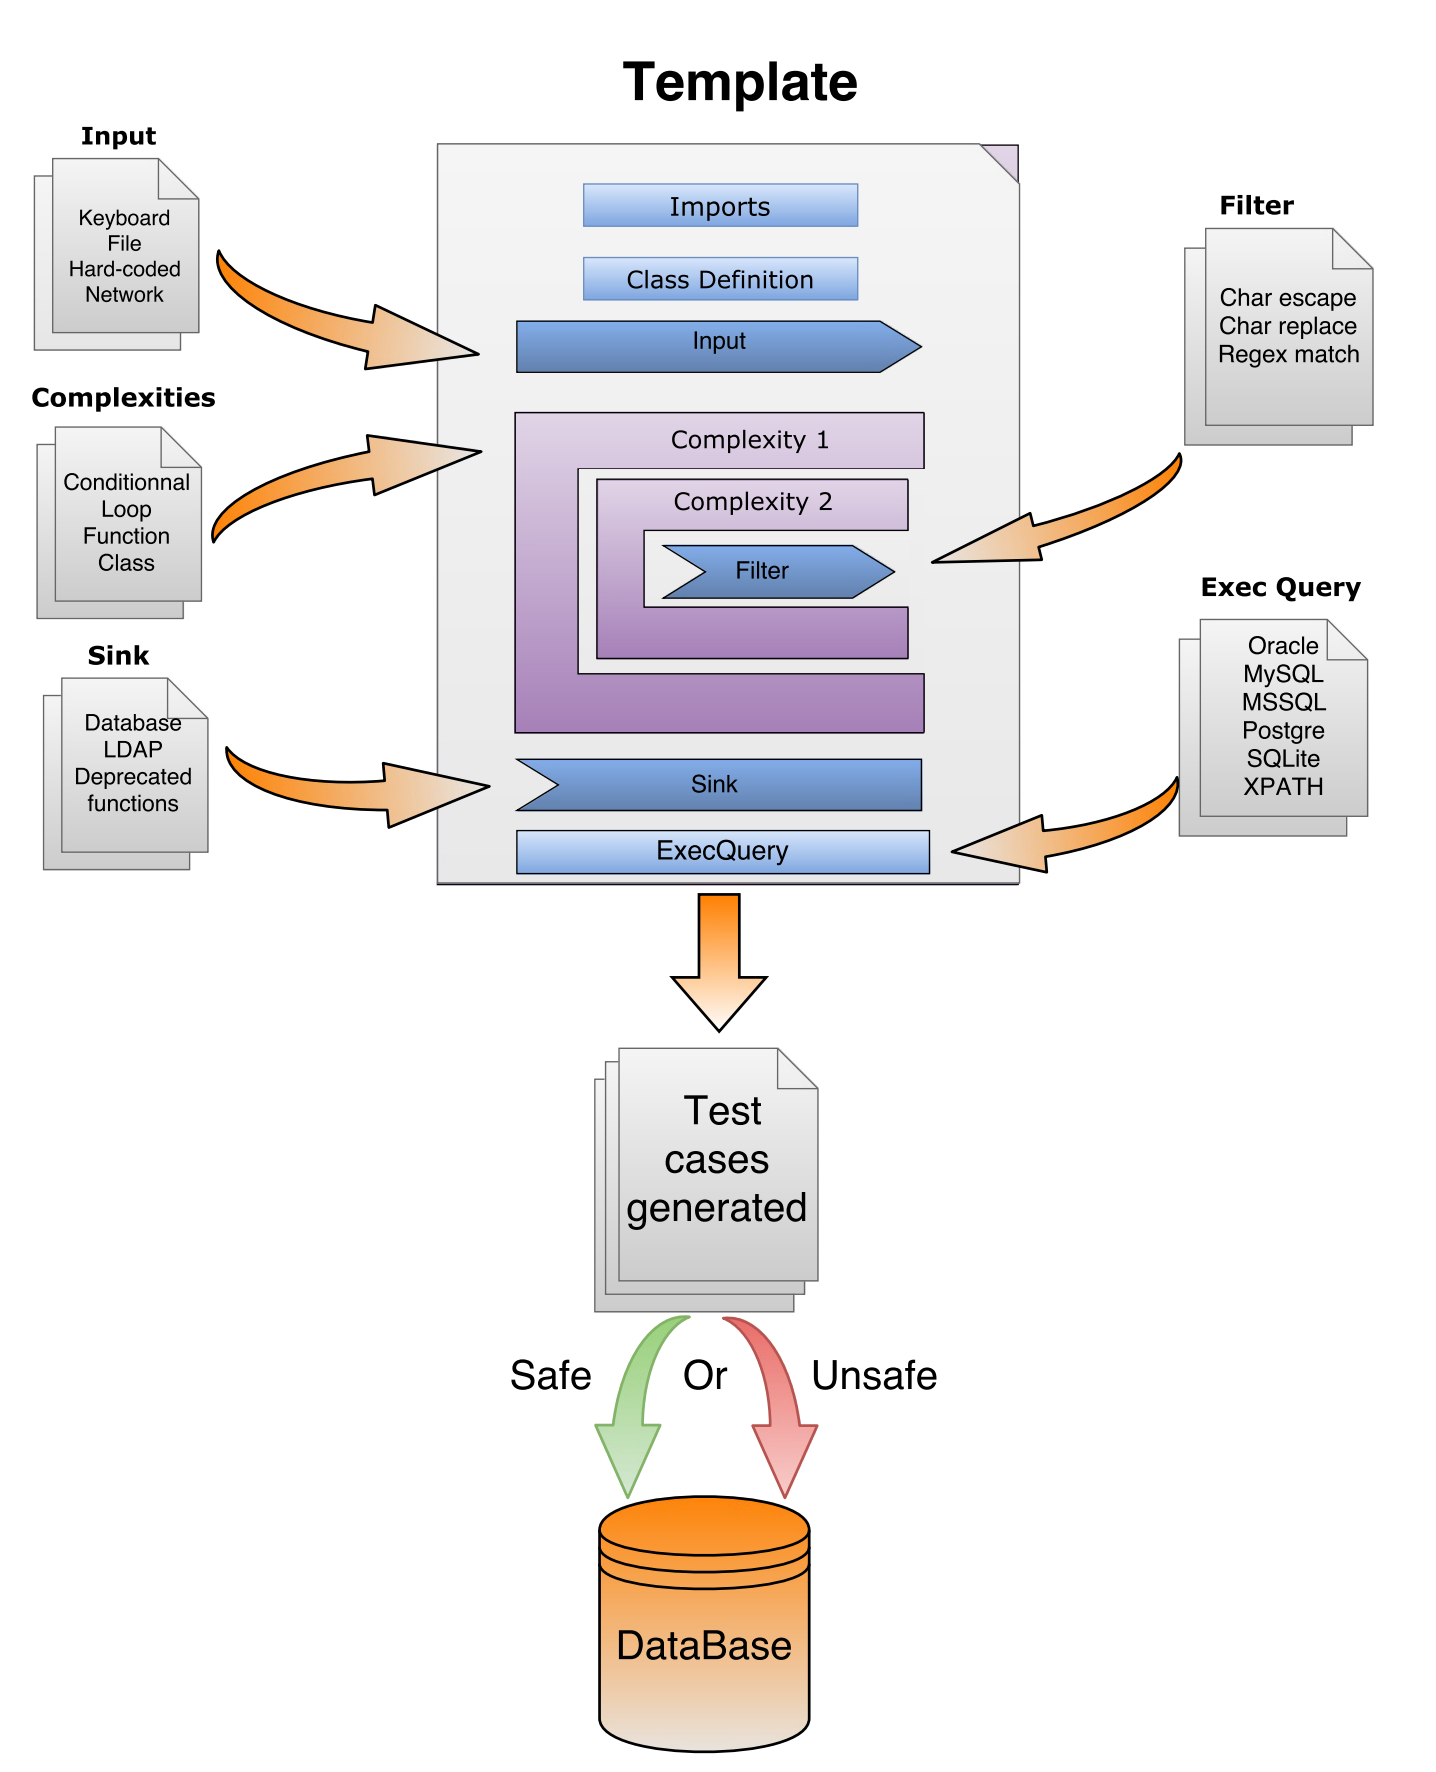
\includegraphics[width=1\linewidth]{fig_VTSG_overview.png}
  \caption{Overview of VTSG test case generation process. The Template
  specifies how pieces are assembled. Input, Filter, Complexity,
  Sink, and ExecQuery modules provide alternative code.  
  An example of
  a generated test case is in 
  Figs.~\ref{fig:example main file} and 
  \ref{fig:example aux file}.}
  \label{fig:VTS operation overview}
\end{figure}

Please note that this document describes two different program structures: the
structure of VTSG itself and the structure of test cases that it generates.

\subsection{Overview of Test Case Generation}

Suppose you write an analyzer to look for bugs in programs.  To test the
analyzer, you need test cases.  Test cases could be lots of many different
programs with lots of different kinds of bugs in different places (and programs
without bugs, too, to test false positives).  It is tedious and error prone to
construct these test cases manually.  VTSG is written to construct huge numbers
of test cases consistently.

In pseudocode, the basic structure of test cases that VTSG generates is
\begin{verbatim}
        declarations
        input = get_input_from_somewhere()
        if input is an attack then
            reject it (filter)
        use the input to make a query (sink)
        execute the query in SQL
\end{verbatim}
You can see this structure in the center rectangle in
Fig.~\ref{fig:VTS operation overview}.

VTSG generates test cases from information in Template, Input,
Filter, Sink, Complexity and ExecQuery files 
(see Fig.~\ref{fig:VTS operation overview}):
\begin{itemize}
 \item Template is the overall structure of each program.
 \item Input is the source of untrusted data in the program, e.g., 
 command line, variable, files, or form methods.
 \item Filter filters the input with functions or methods such as sanitization
   functions, casting, or deprecated functions.
 \item Sink is where a sensitive operation, such as a database query, 
 is executed with potentially untrusted input and where the 
 vulnerability is triggered.
 \item ExecQuery is an additional piece of code that is mandatory to 
 trigger the vulnerability.
 \item Complexities are additional data flow or control flow complications that are
   worked into the structure of the program to exercise tools' abilities.
   Included are conditions inserted into complexities.
\end{itemize}
The content of these files is detailed in
Sec.~\ref{sec:source files}.
Details of the generation process are explained in
Sec.~\ref{sec: generation detail}.

\label{sec:case directory structure}
When invoked to generate test cases, VTSG creates a directory for all the results.
The directory is named for the date and time created, for example,
\verb|TestSuite_03-08-2022_| \verb|16h46m35|.
The language directory, \verb|PHP|,
\verb|Csharp|, or \verb|Python| is created in this directory.
This language name comes from the \verb|name|
in the \verb|file_template.xml| file.  See Sec.~\ref{sec: file template}.

Under the language directory, VTSG creates one directory for each flaw group, for
instance, \verb|OWASP_a1| or \verb|Exception|.  These come from the \verb|flaw_group|
in the \verb|sinks.xml| file; see Sec.~\ref{sec:sink modules}.
Under each flaw group directory is a subdirectory for each specific flaw, for
instance, \verb|CWE78| or \verb|CWE_89|.  These come from the \verb|flaw_type|
entries, which are also in the \verb|sinks.xml| file.
VTSG also creates a manifest file of all the test cases generated for each flaw
group, named
\verb|manifest.xml|.

If the \verb|flaw_group| is missing or empty, subdirectories for flaw types are
created immediately under the language directory.

Under the flaw directory are directories \verb|safe| and \verb|unsafe| for test
cases that are not vulnerable or that are vulnerable respectively.

\subsection{VTSG Directory Structure}
\label{sec: directory structure}

All the language information files are accessed from a single subdirectory.  The
default is \verb|src/templates|.  Another directory may be given with the -t command
line option, see Table~\ref{tab:command line options}.

Under this is one subdirectory for each language.  VTSG chooses the
subdirectory based on the language given in the \verb|-l| command line
option.  Each language subdirectory has six files for that language.
The files are \verb|file_template.xml|, \verb|inputs.xml|,
\verb|complexities.xml|, \verb|filters.xml|, \verb|sinks.xml|,
and \verb|exec_queries.xml|.
The files are described in Sec.~\ref{sec:source files}.
To add another language,
simply create a subdirectory for that language with the six description
files.  See Sec.~\ref{sec:add a language} for more detail.

The \verb|src/templates| directory has \verb|file_rights.txt|, which is
copied into each generated test case to declare license rights and
authorship, see Sec.~\ref{sec: file template}, and a 
\verb|dtd| subdirectory, which has document type definitions (DTDs)
for all of the XML files.


\subsection{Details of Test Case Generation}
\label{sec: generation detail}

Each test case is constructed based on the file template, as shown
in Fig.~\ref{fig:VTS operation overview}. Test cases are 
programs in a specific programming language.
Each test case is generated by
assembling the modules according to the Template.  The
template may direct construction of a simple test case with just
an Input and a Sink.
The Filter code may be embedded in data and control flow
Complexity code.

VTSG generates test cases with two broad steps.  First, VTSG selects
sink, filter, input, exec query, and complexities that are
compatible with each other and consistent with any flaw group or
flaw constraints the user gives on the command line.  Second, VTSG
composes source code from the selected modules, 
synthesizing variable and function names, and writes the file(s).
The user may name an algorithm to choose which cases VTSG composes and writes,
Sec.~\ref{sec:selecting cases}.

VTSG code structure is roughly
\begin{verbatim}
    for each specified sink
        for each filter
            for each input
                for each exec query
                    for up to DEPTH combinations of each complexity
                        save these modules
    for set of saved modules
        compose this set of modules into code for a test case
\end{verbatim}
The code is more complicated because only compatible modules are 
selected.
In addition, some sinks do not need any input or filtering at all,
see Sec.~\ref{sec:sink modules}.
The code is actually structured as a series of function calls to allow types
of modules to be skipped.  Here is a slightly more detailed
overview of those steps, which are in \verb|generator.py|:
\begin{verbatim}
    for each sink:
        if this sink is the type specified:
            use this sink
            if input is needed:
                select_filtering()
            else:
                select_exec_queries()
    
    def select_filtering():
        for each filter:
            if filter is compatible with sink:
                use this filter
                select_input()
    
    def select_input():
        for each input:
            if input is compatible with filter and sink:
                use this input
                select_exec_queries()

    def select_exec_queries():
        if sink needs exec_query:
            for each exec_query:
                if exec_query is compatible with sink:
                    use this exec_query
                    recursion_or_save()
        else:
            recursion_or_save()

    def recursion_or_save():
        if input_type is not none:
            recursive_select_complexity()
        else:
            save_test_case()

    ... and so forth
\end{verbatim}

The \verb|vtsg.py| script creates a new object of the
\emph{Generator} class. 
The program iterates through defined sink modules, selecting those
specified by the user, see
Sec.~\ref{sec:command line interface}, 
or all of them if the user does not specify. It subsequently
selects a compatible filter.  It then goes through all inputs.
The \verb|<input_type>| and \verb|<output_type>|
must be consistent with the ``Filter'' and ``Sink'' XML tags.
Then an exec query and complexities are selected
that are compatible with the currently selected sink module.
See \ref{sec:compatible modules} for details on module compatibility.

When VTSG has selected a set of modules, it saves them as one test case.
Eventually VTSG goes through the list of test cases one by one.  For each one it
composes the code of their modules to generate the source code for a test case.
The process of composing modules to generate source code is
based on XML metadata tags.
After the imports and class definition declaration for the 
specific program
language, the ``Input'' metadata \verb|<code>| portion
is added to the test case.  
The ``Filtering'' metadata \verb|<code>| portion, plus its
\verb|<flaw type>| and safety indicator, are added to
the test case.  Next, the ``Sink'' metadata 
\verb|<code>| portion
is added to the test case.  Finally, the ``ExecQuery'' type is 
noted and the 
\verb|<code>| portion of the ``ExecQuery'' is added
to the 
test case.  The test case is written to one or more files.
The location chosen for the files is
described in Sec.~\ref{sec:case directory structure}.
Section~\ref{sec:case file name} describes how VTSG names the files.

VTSG generates many different test cases, both with and without
flaws, with various control flow complexities.  After VTSG finishes
generating each vulnerability category, it displays how many safe (non-vulnerable)
and unsafe (vulnerable) test cases it produced.
VTSG generates hundreds of test cases in minutes.

VTSG is built to generate test cases with all consistent combinations
of modules for the flaw groups and flaws specified in the invocation.
If VTSG is invoked with particular flaws (\verb|-f|) or flaw groups (\verb|-g|),
only sinks satisfying those specified are used.
If no flaw group is specified, all flaw groups are used.  
If no flaws are specified, all flaws are used.

\label{sec:depth of complexities}
The depth command line option, \verb|-r| or \verb|--depth|, 
specifies the
most nested flow control complexities produced.
VTSG generates test cases with all complexities up to the depth
indicated.
For example, the default depth, 1, leads VTSG to generate all
test cases with no flow complexities and all test cases with 
one complexity.  The option \verb|-r 2| leads VTSG to generate
all cases with no complexities, all cases with one complexity, 
and all cases with two nested complexities.
See Sec.~\ref{sec:code complexities} for an example of three 
nested control flow complexities.

\subsection{Using ACTS to Select a Subset of Cases}
\label{sec:selecting cases}

By default VTSG generates all compatible combinations of inputs, filters, sinks,
exec queries, complexities, and conditions.  The result can easily be tens of
thousands of cases.  Yet, a small, carefully chosen subset of cases may
suffice~\cite{SWInteractions2004}.

ACTS is a combinatorial method to choose cases such that all consistent
pairs or triples or D-way combinations of modules are represented.  For an
explanation of combinatorial testing, see~\cite{KuhnEtAl2010PracCT} especially
Sec. 2.1.

Degree of interaction (doi) is the coverage guaranteed.  Two-way means every
pair of parameter values is represented, like every (allowed) input with every
complexity.  If doi is 3, then every triple is covered, e.g. every input, sink,
and condition combination.  Again only allowed combinations\footnote{The
interface code checks which combinations are actually generated and
writes ACTS constraints to \emph{not} create combinations that never occur.
For instance, one filter, named ``none'', just passes the input value; it
doesn't filter anything.  The filter is marked as need\_complexity="0" (See
Sec.~\ref{sec:need complexity}), to avoid wrapping it in any complexity: it
would useless to wrap an if or while around it.  The interface code sees that
filter ``none'' never has complexities, so constrains ACTS to only match that
filter with ``no complexity''.
}
are created.  The default is for ACTS to generate pairwise coverage, that is,
the default degree of interaction is two.

For example,
\begin{verbatim}
$ python3 vtsg.py -l php --ACTS
\end{verbatim}
generates a small set of PHP test cases that have all pairs of compatible
modules.
\begin{verbatim}
$ python3 vtsg.py -l py -g Exception --ACTS,4
\end{verbatim}
generates a small set of Python test cases that have all 4-way combinations of
compatible modules in the \verb|Exception| flaw group.
If ACTS should select a combination of modules that was not generated, VTSG
halts with an error message.

VTSG first generates all consistent combinations of modules,
Sec.~\ref{sec: generation detail}.  If \verb|ACTS| is indicated, VTSG writes
the list of modules and constraints on compatible modules to
\verb|/tmp/VTSG_ACTS_input.xml|, runs ACTS, reads the selected sets of modules
from \\ \verb|/tmp/VTSG_ACTS_output.txt|, and creates a list of matching module
combinations.  VTSG then composes the code from modules and writes the test
cases.

Currently, the code to write input for ACTS and read its output does \emph{not}
handle more than one complexity in a case.  Therefore, \verb|-r| (depth) and
-\zws-ACTS may not be used together.  It should be straight forward to enhance
the code, which is in \verb|select_by_acts.py|, to handle any number of
complexities.

The -n option is another way to select which cases VTSG should write.
Therefore, -n and -\zws-ACTS are mutually exclusive.

\subsection{Code Complexities}
\label{sec:code complexities}

In theory, a static analysis tool only needs to process a few lines of
code that
embody the vulnerability. In practice, a tool must analyze much
of the program,
noting its control and data flows, to accurately track data and
determine the
conditions when the code with weaknesses may be executed.
Tracing execution through structures like \verb|while| loops, \verb|if|
statements, and function calls may confuse static analysis tools.
We refer to these constructs as code complexities.
VTSG can nest code complexities to create slightly more realistic source code.

The complexities currently defined
are listed in the appendixes for their languages.

Here is an example of code complexities from \verb|cwe_89__I_shell_commands__F_no_|\\
\verb|filtering__S_select_from-concatenation_simple_quote__EQ_mysql| \\
\verb|__3-2.5-9-21a.cs|: \\
{\texttt
{\colorbox{yellow}{if((Math.Pow(4, 2)<=42))\{}}\\
\hspace*{2em}{\colorbox{green}{switch(6)\{}}\\
\hspace*{4em}{\colorbox{green}{case(6):}}\\
\hspace*{6em}{\colorbox{cyan}{Class\_8 var\_8 = new Class\_8(tainted\_5);}}\\
\hspace*{6em}{\colorbox{cyan}{tainted\_6 = var\_8.get\_var\_8();}}\\
\hspace*{6em}tainted\_7 = tainted\_6;\\
\hspace*{6em}{\colorbox{green}{break;}}\\
\hspace*{4em}{\colorbox{green}{default:}}\\
\hspace*{6em}{\colorbox{green}{break;}}\\              
\hspace*{2em}{\colorbox{green}{\}}}\\
{\colorbox{yellow}{\}else\{}}\\
\hspace*{2em}{\colorbox{yellow}{\{\}}}\\
{\colorbox{yellow}{\}}}
}
\\
The above has three nested control structures:\\
{\colorbox{yellow}{Level 1 is the ``if'' statement.}}\\
\hspace*{2em}{\colorbox{green}{Level 2 is the ``switch'' statement.}}\\
\hspace*{4em}{\colorbox{cyan}{Level 3 is the call of a method from a Class.}}


\section{Template, Input, Filter, Sink, Exec\_Query, and Complexity Files}
\label{sec:source files}

These XML files are required for each language.
There 
are a few XML-specific caveats that must be paid attention to when 
creating these files. 
Table~\ref{tab:XML escapes} lists the symbols that may cause errors 
during the process and the XML equivalent replacement necessary to 
complete the
task without error.

\begin{table}[H]
\centering
\caption{Replacement sequences for characters that are treated 
in a special way in XML files.}
\begin{tabular}{|c|l|}
\hline
\textbf{Character} & \textbf{Replacement} \\
\hline
 \verb|<| & \&lt; \\
\hline
 \verb|>| & \&gt; \\
\hline
 \verb|"| & \&quot; \\
\hline
 \verb|'| & \&apos; \\
\hline
 \verb|&| & \&amp; \\
\hline
\end{tabular}
\label{tab:XML escapes}
\end{table}

VTSG uses Jinja to compose code. In addition to the above, Jinja recognizes
double-curly-brackets (\{\{ and \}\}) as introducing Jinja-specific variables and
controls.  Do not use pairs of curly brackets in your files, except for VTSG-related
variables.

Characteristics of modules and their information are stored in 
XML files.  
This section of the document describes the structure of each type of module and
the meaning
of each element and its tags.

Most of the file types have an example followed by
an explanation of what it does and what it generates.

Each language directory has one file of each name. That is,
one \verb|file_template.xml| file, one \verb|inputs.xml| file,
one \verb|filters.xml| file, one \verb|complexities.xml| file,
one \\ \verb|sinks.xml| file, and one \verb|exec_queries.xml| file.

All the files, except \verb|file_template.xml|, may have many
modules, that is alternate chucks of code, in them.
For example, \verb|inputs.xml|, Sec.~\ref{sec: input module}, typically has many input
modules.  Each module in \verb|inputs.xml| provides a method to get input from a
different source, such as command line options or hard-coded values.

\subsection{Maintain Indentation with INDENT ... DEDENT}
\label{sec:indent}

VTSG using Jinja does a haphazard job of producing proper indentation.  Indentation
does not matter for many languages.  It is critical for Python, however.  This
section explains how to use INDENT and DEDENT to ensure correct indentation in the
final source code.

\subsubsection{Using INDENT ... DEDENT}
INDENT ... DEDENT sections may appear in any of the above files.  They
most often occur in \verb|file_template.xml| and \verb|complexities.xml| files.

Use INDENT and DEDENT lines in code chunks to indicate that
any code between those lines should be indented consistently.  For example,
\begin{verbatim}
def main():
INDENT
    {{local_var}}
    {{input_content}}
    {{filtering_content}}
    {{sink_content}}
    {{exec_queries_content}}
DEDENT
\end{verbatim}
All code produced from the statements between the INDENT/DEDENT lines is
consistently indented with the string defined in \verb|<indent>| \verb|</indent>|,
which appears in \\ \verb|file_template.xml|, see Sec.~\ref{sec: file template}.
That string is typically four spaces.

INDENT sections may be nested.  For example, here is a sink module with code that
needs additional indentation.
\begin{verbatim}
        print(f'file "{ {{in_var_name}} }" ', end='')
        {{flaw}}
        if os.path.exists({{in_var_name}}):
	INDENT
            print('exists')
	DEDENT
        else:
	INDENT
            print('does not exist')
	DEDENT
\end{verbatim}
If the INDENT lines were not included, VTSG produces the following code (slightly
edited for presentation).
\begin{verbatim}
def main():
    tainted_0 = input()
    tainted_1 = tainted_0
    
        # No filter (sanitization)
        tainted_1 = tainted_0
            
    
        print(f'file "{ tainted_1 }" ', end='')
        #flaw
        if os.path.exists(tainted_1):
            print('exists')
	else:
            print('does not exist')
\end{verbatim}
Notice that the indentation is not consistent. This is not valid Python code.
With INDENT lines, VTSG produces the following, which is valid Python.
\begin{verbatim}
def main():
    tainted_0 = input()
    tainted_1 = tainted_0

    # No filter (sanitization)
    tainted_1 = tainted_0


    print(f'file "{ tainted_1 }" ', end='')
    #flaw
    if os.path.exists(tainted_1):
        print('exists')
    else:
        print('does not exist')
\end{verbatim}


\subsubsection{Details of INDENT ... DEDENT}

Here are details of using INDENT and DEDENT.

VTSG processes code within INDENT sections line by line. No semantic parsing or
analysis is done.

A section to be fixed is indicated by a line beginning with \verb|INDENT|, possibly
with leading whitespace. The end of the section is indicated by a line beginning with
\verb|DEDENT|, again possibly with leading whitespace. Any text after INDENT or
DEDENT to the end of the line is ignored.

Indent sections may be nested.

INDENT and DEDENT lines are removed.
For lines within an INDENT ... DEDENT section,
\begin{itemize}[nosep]
\item first, any leading whitespace is removed, and
\item second, if the line is not empty, indentation is added for each nested
  INDENT ... DEDENT section this is in.
\end{itemize}

Here is a convoluted example to illustrate the fine points.  Suppose this is the
code generated by composing the modules.
\begin{verbatim}
      if Condition:
INDENT            text after INDENT is ignored
           line 1
               while not True:
          INDENT
           line 3 - INDENT not at the beginning is ignored
     DEDENT

                  line above is empty
        DEDENT
        line 5
\end{verbatim}
If the indent string is specified as \verb|<indent>..,</indent>|, the following is
the result. (Note: typically, the indent is four spaces. The preceding string with
periods and a comma is only for example clarity.)
\begin{verbatim}
      if Condition:
..,line 1
..,while not True:
..,..,line 3 - INDENT not at the beginning is ignored

..,line above is empty
        line 5
\end{verbatim}

Note: because \emph{all} leading whitespace is removed from lines in indent sections,
using INDENT ... DEDENT anywhere means that every indentation must be indicated
with INDENT ... DEDENT lines.

We chose ``DEDENT'' because it is used in Python's grammar description.


\subsection{File Template}
\label{sec: file template}

\begin{verbatim}
<template type="" name="">
    <file_extension></file_extension>
    <comment>
        <open></open>
        <close></close>
        <inline></inline>
    </comment>
    <syntax>
        <statement_terminator></statement_terminator>
        <indent></indent>
    </syntax>
    <namespace></namespace>
    <variables prefix="" import_code="using {{import_file}};">
        <variable type="" code="" init=""/>
    </variables>
    <imports>
        <import></import>
    </imports>
    <code></code>
</template>
\end{verbatim}

\begin{itemize}
    \item name: Programming language name, e.g., PHP, Csharp,
    or Python. This appears in the manifest.
    It is also the name of the subdirectory under the TestSuite directory
    where all the generated test cases are placed.

    \item file\_extension: Extension of the generated files.

    \item comment: Strings indicating comments.
    \begin{itemize}
        \item open: string to begin a comment, which may span many lines
        \item close: string to end a comment, which may span many lines
        \item inline: string to begin a one-line comment
    \end{itemize}
    
    \item syntax: Other language-specific syntax.
    \begin{itemize}
        \item statement\_terminator: string to show the end of 
        a statement.
        This is semicolon
        \verb|<statement_terminator>;</statement_terminator>|
        in PHP, C, Java, \\ and \CSharp. Python does not have 
        a terminator, so this is the empty string: \\
        \verb|<statement_terminator></statement_terminator>|.

        \item indent: string used to indent code, see Sec.~\ref{sec:indent}.
          This is typically four spaces, but
          can be any string.
    \end{itemize}
    
    \item namespace: Namespace name, if applicable

    \item variables: Information about variable names and types and how
    to include libraries.
    \begin{itemize}
        \item prefix: Any prefix required for variable names.
        \$ for PHP.
        Leave it empty if not required.

        \item import\_code: Code to include a library. The code
        should have the placeholder \verb|{{import_file}}|.
        For example, \verb|#include <{{import_name}}>|.
        
        \item variable: Defines each variable type and how to initialize it. (optional)
        \begin{itemize}
        \item type: Names the type. This string 
        does not appear in the test case code.  It tells VTSG
        the type of variable that is being used.  The input\_type
        and output\_type in Input, Filter, and Sink modules use
        this string.

        \item code: A piece of code to declare the type of the variable. For
        some languages, such as PHP and Python, this field can be blank. 
        This value gives the variable type when being declared, for example,
        \verb|string var_0;|.  In this case, ``string''
        is the value put in this attribute.

        \item init: Value assigned when this type of variable is initialized.
        \end{itemize}
        If variables do not need to be declared in this language, do not include
        any \verb|<variable ... />| statements or the \verb|{{local_var}}|
        placeholder in the code.
    \end{itemize}
    
    \item code: the template code. It should contain the 
    following placeholders:
    \begin{itemize}
        \item comments: This is replaced by comments in the selected input,
        filter, sink, and exec query modules.  This is intended to
        describe the variants, options, and use of this test case. 
        
        \item license: This is replaced by the contents of the
        \verb|file_rights.txt| file.  This is intended to hold
        authors' names, usage and copyrights, contact information, 
        etc.
        
        \item stdlib\_imports:  This is a placeholder for
        \emph{all} imports for the generated program

        \item namespace\_name:  Used if the language requires it

        \item main\_name:  Name of the main class

        \item local\_var: Location to declare local variables (optional).  If
          variables do not need to be declared in this language, do not include this
          placeholder or any \verb|<variable ... />| statements in the variables.

        \item input\_content:  Location for the Input (required)

        \item filtering\_content: Location of the Filter, which will be wrapped with
          complexities, if any.

        \item sink\_content:  Location for the Sink

        \item exec\_queries\_content:  Location for the ExecQuery

        \item static\_methods:  Location for the static functions.
    \end{itemize}
\end{itemize}


\subsection{Attributes Shared By Modules}
\label{sec:shared attributes}

Many kinds of modules use the same attributes.  Instead of repeating explanation of
these attributes, they are here.

\subsubsection{Module Description in Path and Dir Tags}
\label{sec:module description}

Within the \verb|<path>| keywords, modules may have one or more \verb|<dir>| tags.
These tags provide the descriptions of the module that is used in the file name, see
Sec.~\ref{sec:case file name}.  For example, when the key word in a selected input
module is ``file'', the file name will contain \verb|..._I_file_...|, where ``I''
indicates the input module selected.

If a module has more than one \verb|<dir>| tag, the strings are joined with dashes.
For example, if a sink has
\begin{verbatim}
            <path>
                <dir>select_from</dir>
                <dir>concatenation_simple_quote</dir>
            </path>
\end{verbatim}
then cases using that module will have file names containing \\
\verb|_S_select_from-concatenation_simple_quote_|.

Note: we cannot think of any reason why it is better to give multiple description
strings instead of just one string.  But the functionality is provided in VTSG, and
some modules use it.


\subsubsection{Module Comment}
\label{sec:module comment}

If a sample module has a comment string, it is added to the
\verb|{{comments}}| area in the file template, Sec.~\ref{sec: file template}.
This informs the user about the purpose or structure of the input, filter, sink, and
exec query modules included.  Below is an example comment string.

\begin{verbatim}
            <comment>sink: check if a file exists</comment>
\end{verbatim}

Any case using that module will have
\begin{verbatim}
sink: check if a file exists
\end{verbatim}
in the comments area.


\subsubsection{Needed Imports}
\label{sec:module import}

Sometimes the use of code requires some library to be imported or used.  This is
indicated with names in \verb|<import></import>| directives within
\verb|<imports></imports>| sections.

Code statements are synthesized from the \verb|import_code| in the file template and
the name or names given here.


\subsubsection{Marking Modules as Safe and Unsafe}
\label{sec:safe or unsafe}

Using some modules in a program for certain flaws may make them safe or may make them
unsafe.  For instance, prepared SQL statements are always safe from SQL injection
vulnerabilities.  In contrast using a broken cryptographic algorithm is always
unsafe, regardless of how any user input is filtered.  Similarly certain
hard-coded inputs may always make a program safe from certain flaws, and some filters
may make a program safe from certain flaws for any user input.

Input, filter, and sink modules can be marked as always safe or always unsafe using
\verb|safe="1"| or \verb|unsafe="1"|.  Modules may be always safe or always unsafe
(or neither) for some flaws and have different safety attributes for other
flaws.

Exec query modules may be marked as always safe.  (No exec query module can make the
program unsafe.)

A generated program is not safe if any of the selected input, filter, or sink modules
are always unsafe, that is \verb|unsafe="1"|.  A program is safe if any of the
selected input, filter, sink, or exec query modules is always safe, that is
\verb|safe="1"|, \emph{and} none
are unsafe.  If no module is safe, the generated program is unsafe.
The filter module must be executed to be considered.  In other words, if
a complexity never executes the filter, then the filter's safe or unsafe marking is
ignored.  Table~\ref{tab:selection safe algorithm} expresses this as a table.

\begin{table}[H]
\centering
\caption{Decision table for whether a set of modules is safe or unsafe.}
\begin{tabular}{c|c|c|}
  & \makecell{Any module \\ has safe="1"}
  & \makecell{No module is \\ always safe} \\
\hline
\makecell{Any module \\ has unsafe="1"}  & not safe & not safe \\
\hline
\makecell{No module is \\ always unsafe} &   safe   & not safe \\
\hline
\end{tabular}
\label{tab:selection safe algorithm}
\end{table}

The Code Complexity Modules, Sec.~\ref{sec: complexity modules}, explains when a
filter may never be executed.


\subsection{Input Modules}
\label{sec: input module}

The \verb|inputs.xml| file has one or more ``sample'' input modules.  Each module
provides one way for the generated program to get input.

\begin{verbatim}
<sample>
    <path>
        <dir></dir>
    </path>
    <comment></comment>
    <flaws>
        <flaw flaw_type="" [safe=""] [unsafe=""]/>
    </flaws>
    <imports>
        <import></import>
    </imports>
    <code></code>
    <input_type></input_type>
    <output_type></output_type>
</sample>
\end{verbatim}

\begin{figure}[htb]
  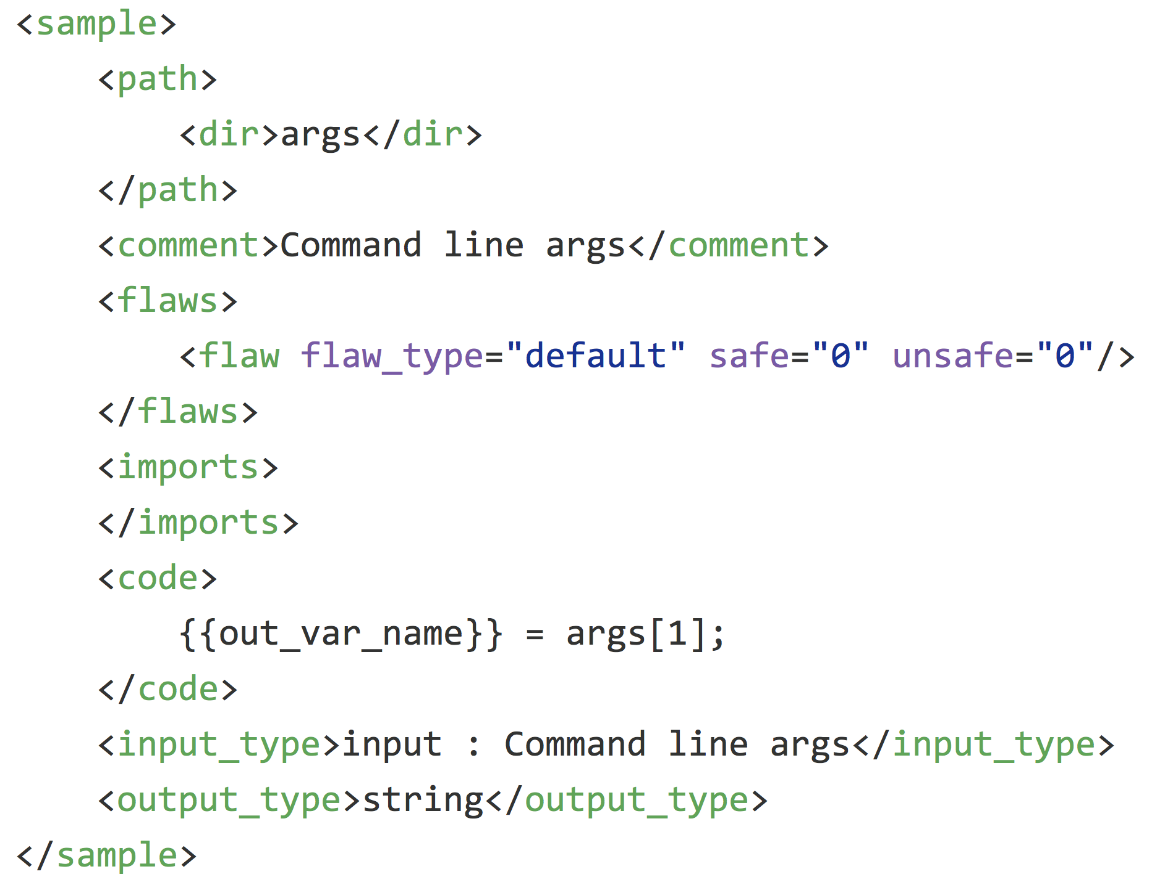
\includegraphics{fig_Input_file.png}
  \caption{Example Input module.  Instantiated at line 14 of 
  Fig.~\ref{fig:example main file}.}
  \label{fig:example input file}
\end{figure}

\begin{itemize}
    \item dir and path, comment, and imports: see Sec.~\ref{sec:shared attributes}.

    \item flaw: may indicate whether this input is always safe or always unsafe.
      See Sec.~\ref{sec:safe or unsafe} for
      more details.  If this input has the same safe/unsafe value for most
      types of vulnerabilities, put ``default'' as the \verb|flaw_type|.

    \item input\_type: this string is placed in the manifest.  It has no other
      function in VTSG.

    \item output\_type: the type of output.  The variable generated with the
      placeholder \\ \verb|{{out_var_name}}| in the code will be that type.
      An input module is selected if it matches the \verb|input_type| of the Filter
      (or of the Sink, if the Filter \verb|input_type| is ``nofilter'').

    \item code: The source code of an input. It should contain the placeholder \\
      \verb|{{out_var_name}}|.  That placeholder will be replaced by the variable
      name used in the Filter and Sink.  Do not declare this variable.
\end{itemize}

The case generated from the example Input in 
Fig.~\ref{fig:example input file}
takes an argument from the command line as Input.  
The input string can be either safe or unsafe, depending on user input.

\subsection{Filter Modules}

All filter modules are in the \verb|filters.xml| file.

\begin{verbatim}
<sample>
    <path>
        <dir></dir>
    </path>
    <comment></comment>
    <flaws>
        <flaw flaw_type="" [safe=""] [unsafe=""]/>
    </flaws>
    <imports></imports>
    <code></code>
    <input_type></input_type>
    <output_type></output_type>
    <options need_complexity=""/>
</sample>
\end{verbatim}

\begin{figure}[htbp]
  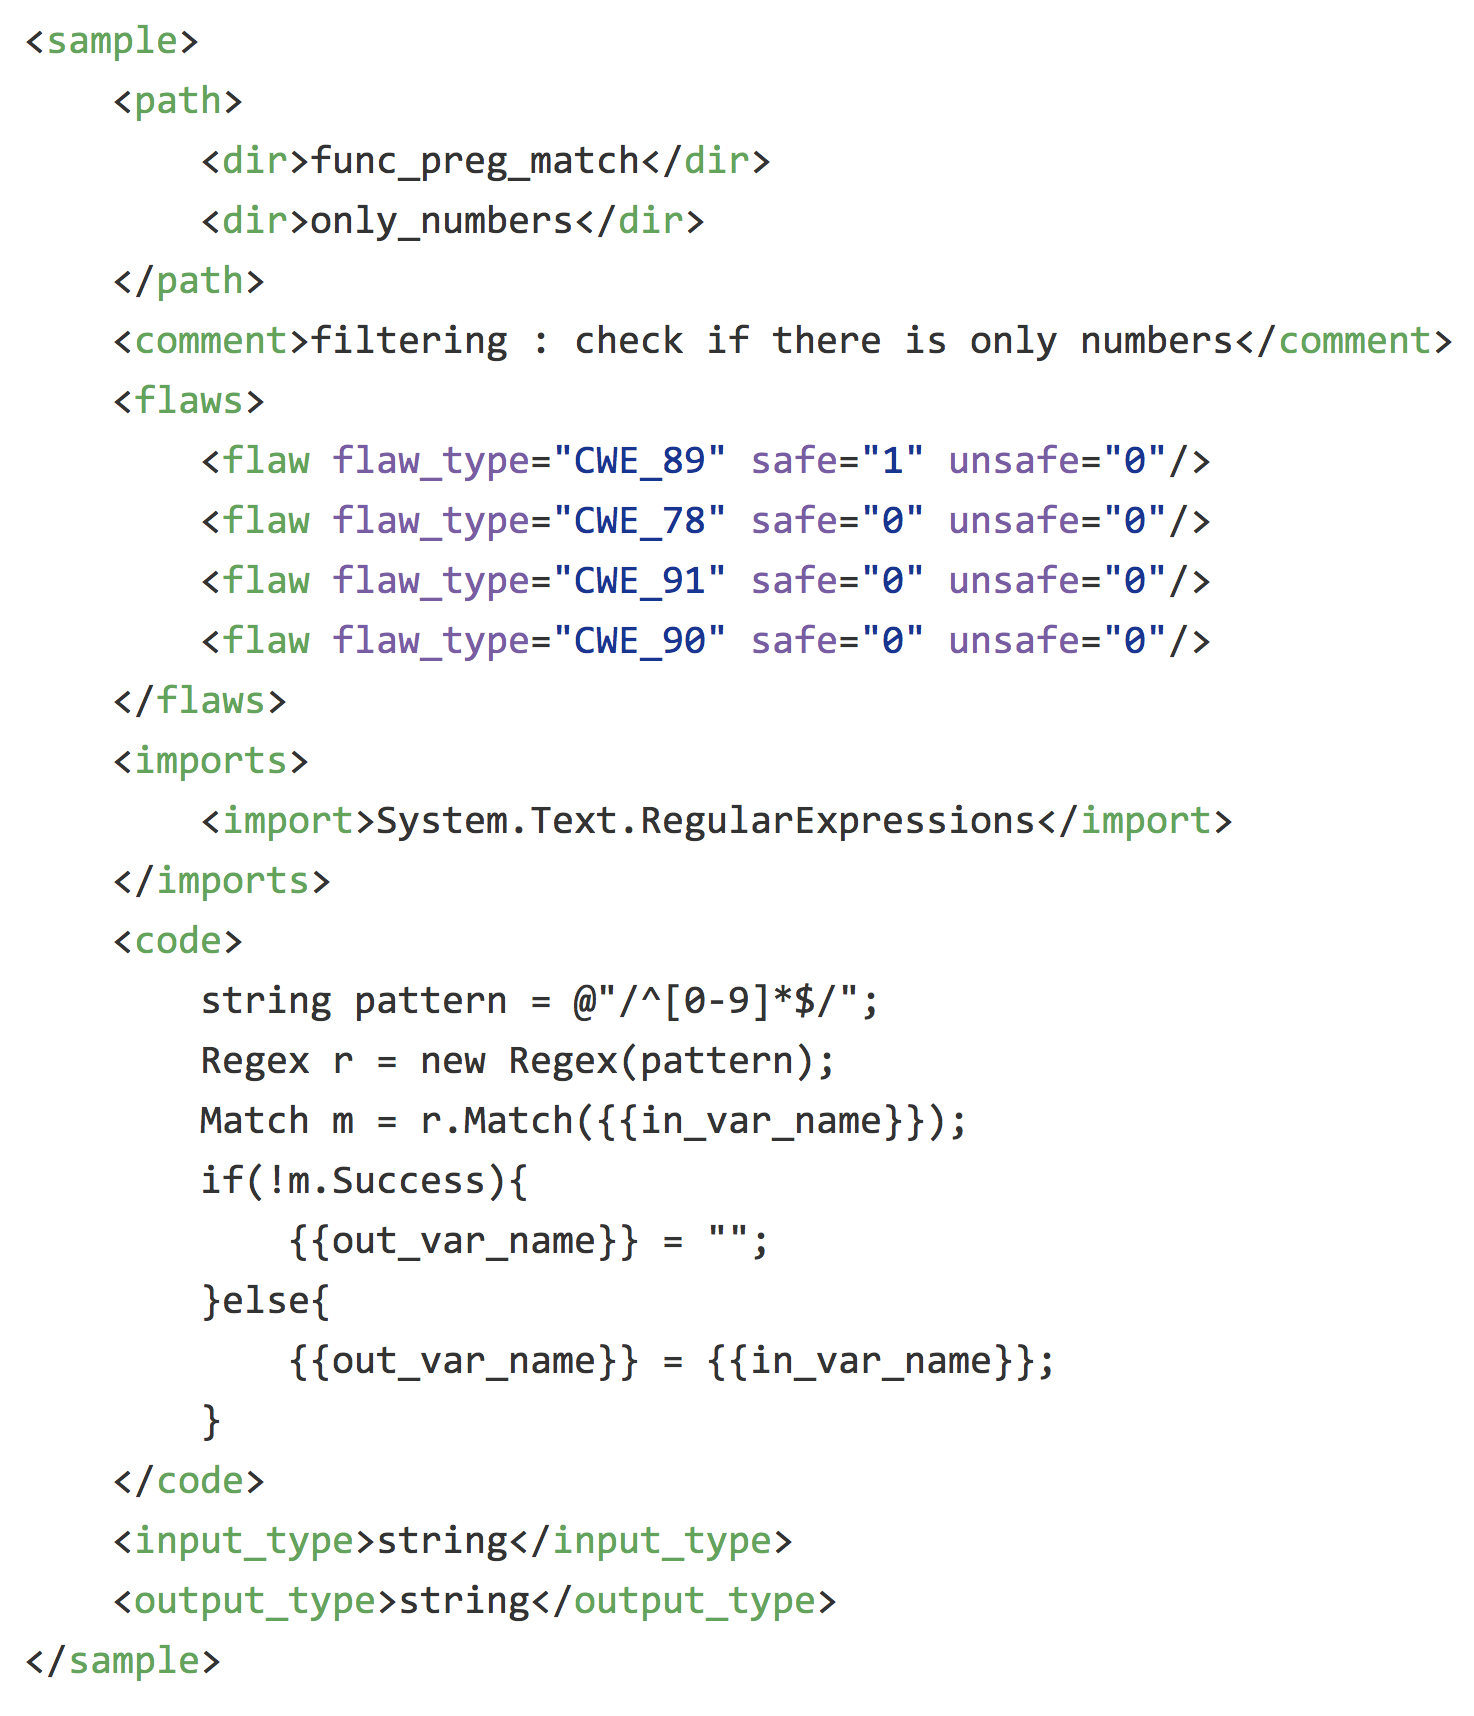
\includegraphics[width=\linewidth]{fig_Filter_file.png}
  \caption{Example Filter module. Instantiated in lines 19--27 of
           Fig.~\ref{fig:example aux file}.}
  \label{fig:example filter file}
\end{figure}

\begin{itemize}
    \item dir and path, comment, and imports: see Sec.~\ref{sec:shared attributes}.

    \item input\_type: the input type of the filter. The variable 
    generated with
    the placeholder \verb|{{in_var_name}}| will be that type.
    Declarations of \verb|variable| in the File Template give
    available types, see Sec.~\ref{sec: file template}.

    \item output\_type: the output type of the filter.  The variable generated
    with the placeholder \verb|{{out_var_name}}| will be that type.

    \item flaw: indicate whether this filter is always safe, always unsafe, or
      neither for a particular flaw type.  See Sec.~\ref{sec:safe or unsafe} for
      more details.  If this filter has the same safe/unsafe value for most
      types, put ``default'' as the \verb|flaw_type|.

    \item code: The source code of a filter. It should contain the placeholders
    \\
    \verb|{{in_var_name}}| and \verb|{{out_var_name}}|.  Those placeholders will 
    be replaced by the variable names that will be used in the Input and in Sink.  Do
    not declare these variables.
    \verb|{{out_var_name}}| must receive a value in all possible executions of the
    filter.
    \\
    Tip: To generate a test without functional filtering, just assign
    \verb|out_var_name| the value of \verb|in_var_name|, e.g.,
\begin{verbatim}
    {{out_var_name}} = {{in_var_name}};
\end{verbatim}
    and make the input\_type and output\_type \verb|nofilter|.
    This passes the value from the Input directly to the Sink.

    \item options: By default filters are wrapped in complexities.  Complexities may
      be disabled by adding \verb|options| with \verb|need_complexity="0"|.
      \label{sec:need complexity}
      In other words, if \linebreak[4] \verb|need_complexity| is in
      \verb|<options />| with anything other than ``1'', VTSG does not generate any
      variations with complexities.
\end{itemize}

The example Filter file in Fig.~\ref{fig:example filter file} makes sure
the Input contains only a number.  
The flag safe is 1, because you cannot cause an SQL Injection 
(CWE 89) with only numbers.


\subsection{Sink Modules}
\label{sec:sink modules}

All sink modules are in the language's \verb|sinks.xml| file.

\begin{verbatim}
<sample>
    <path>
        <dir></dir>
    </path>
    <flaw_type flaw_group=""></flaw_type>
    <safety safe="" unsafe=""/>
    <comment></comment>
    <imports>
        <import></import>
    </imports>
    <code></code>
    <input_type></input_type>
    <exec_type></exec_type>
</sample>
\end{verbatim}

\begin{itemize}
    \item dir and path, comment, and imports: see Sec.~\ref{sec:shared attributes}.

    \item flaw\_type: the flaw\_group is a general category of vulnerability.
    Generated test cases are placed under the flaw group subdirectory, then
    in the flaw type subdirectory under that.  If the flaw\_group is missing or
    empty, flaw type subdirectories are created immediately under the language
    directory.
    The user can limit
    cases generated to certain flaw groups with \verb|-g| command
    line options or certain flaws with \verb|-f| options.
    
    \item input\_type: the input type of the sink. The variable
    generated with the placeholder \verb|{{in_var_name}}| will be 
    that type.  If the sink does not
    require an input, this type should be \verb|none|. The code 
    should not contain
    the placeholder \verb|{{in_var_name}}|.
    Declarations of \verb|variable| in the File Template give
    available types, see Sec.~\ref{sec: file template}.

    The input type specifies the kind of data this sink needs from the filter (or
    from the input).  VTSG only selects filters whose output types are the same as
    this input type.  If the filter input type is ``nofilter'',
    then VTSG selects input modules whose
    output types are the same as this input type.

    \item exec\_type: link a sink to the exec queries.  It must have 
    the type of
    an ExecQuery. If it does not require an ExecQuery, 
    exec\_type should be \verb|none|.

    \item safety: whether the sink is always safe or always unsafe.  For instance, a
      deprecated function may be marked (always) unsafe.
      See Sec.~\ref{sec:safe or unsafe}
      for more details.
    
    \item code: The source code of a sink. It should contain the placeholder
    \verb|{{in_var_name}}|.  The placeholder will be replaced by the variable
    name used in the Filter.  Do not declare this variable.

    The placeholder \verb|{{flaw}}| indicates that the next line is the location
    of the flaw.  In other words, if this case is unsafe, the manifest reports a
    flaw at the line following this.  In generated unsafe cases,
    \verb|{{flaw}}| is replaced with the one-line comment string,
    see Sec.~\ref{sec: file template}, and ``flaw''.
    It does not appear in generated safe cases.
\end{itemize}

\begin{figure}[htbp]
  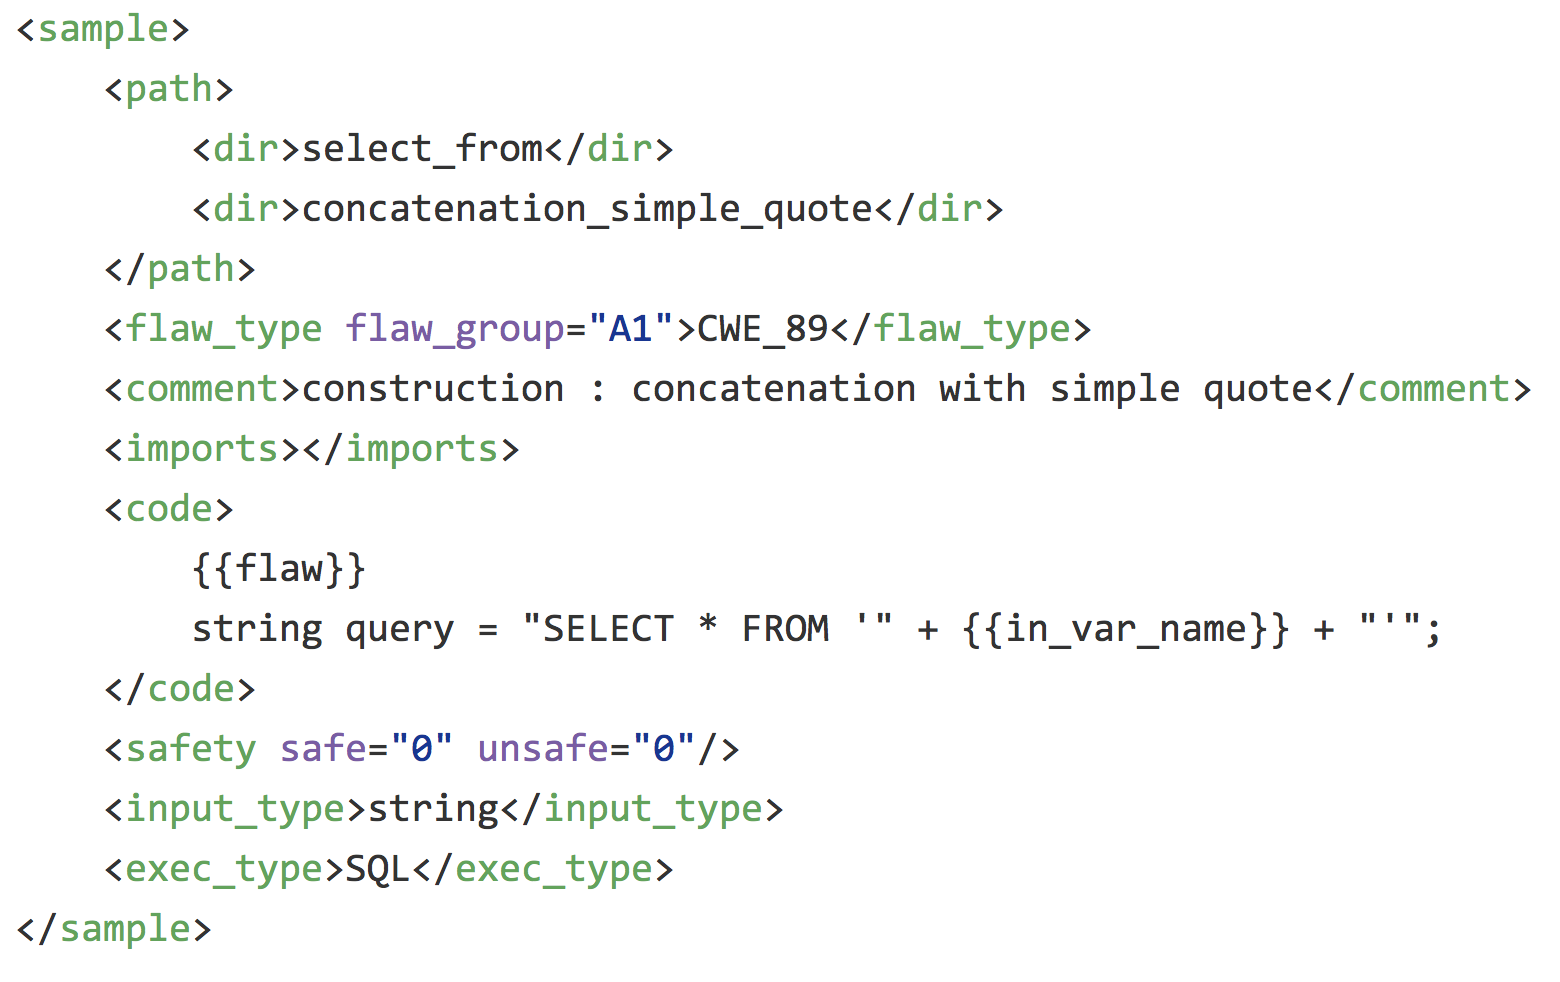
\includegraphics[width=\linewidth]{fig_Sink_file.png}
  \caption{Example Sink module. Instantiated at line 23 of
           Fig.~\ref{fig:example main file}.}
  \label{fig:example sink file}
\end{figure}

The Sink example in Fig.~\ref{fig:example sink file} 
concatenates the filtered string with an SQL query.  This block
of code can only be used for SQL Injection.  Whether or not it is
vulnerable depends on the input string.


\subsection{Exec\_Query Modules}

All query execution modules are in the language's \verb|exec_query.xml|
file.

\begin{verbatim}
<exec_query type="" safe="">
    <path>
        <dir></dir>
    </path>
    <comment></comment>
    <imports>
        <import></import>
    </imports>
    <code></code>
</exec_query>
\end{verbatim}

\begin{itemize}
    \item type: the type of the ExecQuery. This is used in the
    \verb|exec_type| tag of the Sink to link them together during
    generation process.  The type should only contain letters, numerals, and
    underscore (``\_'').\\
    Languages currently available for VTSG support many database management
    systems, including ORACLE, MySQL, MSSQL, PostgreSQL, SQLite, and XPATH.
    The syntax of each ExecQuery must be
    compatible with its associated database system language.
    
    \item safe: whether the ExecQuery always makes the case safe.
    See Sec.~\ref{sec:safe or unsafe} for more details.

    \item dir and path, comment, and imports: see Sec.~\ref{sec:shared attributes}.

    \item code: The source code of a query. It does not contain placeholders.
    It should be linked to the corresponding variable from the Sink. The linking is done through the "exec\_type" attributes within the XML files.
\end{itemize}


\begin{figure}[htbp]
  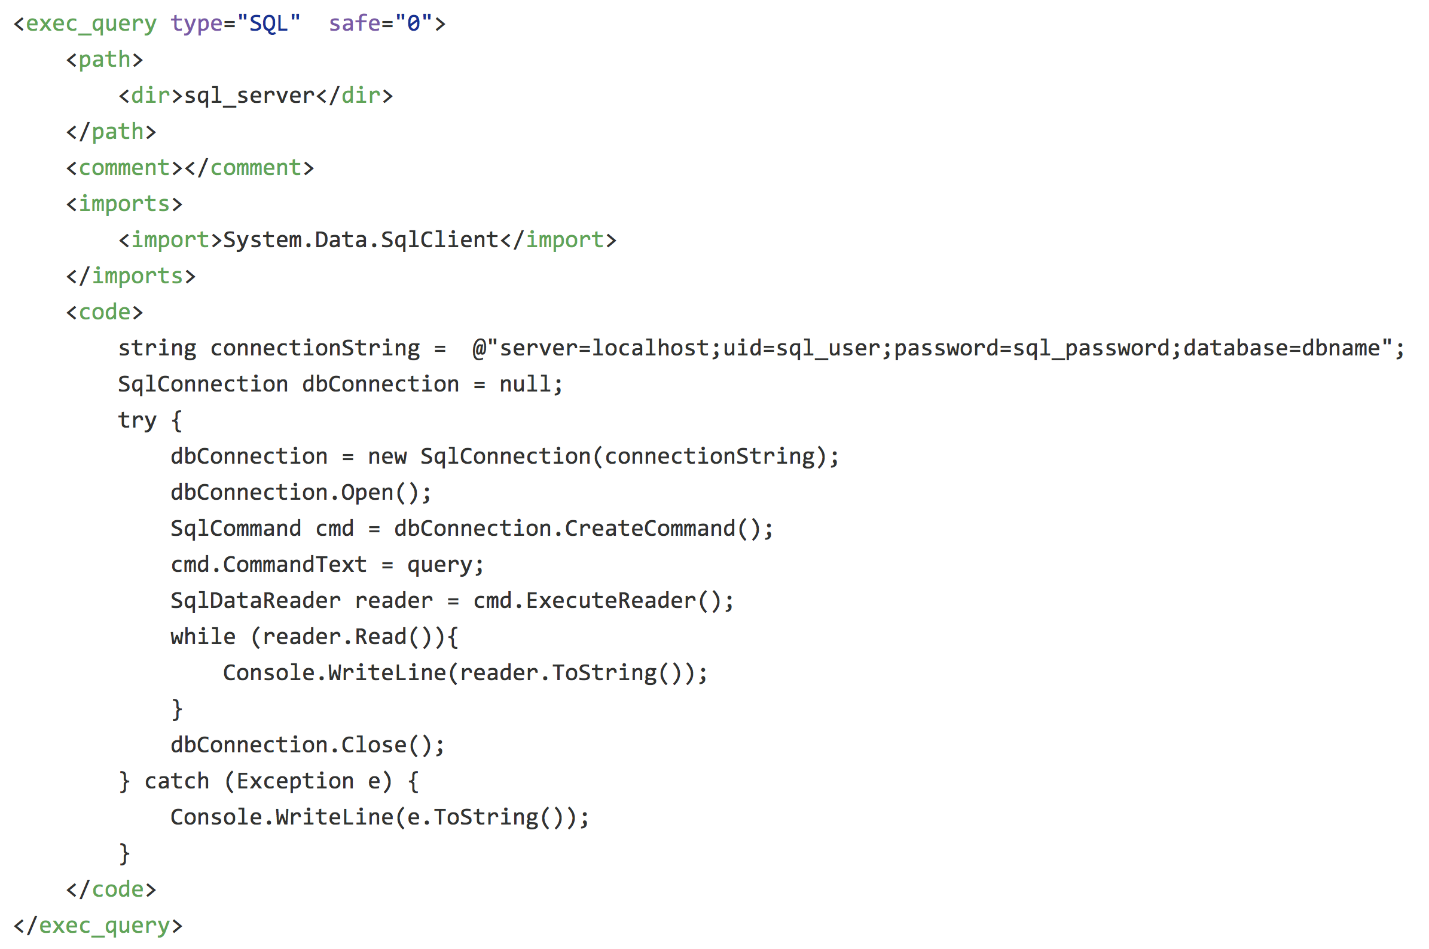
\includegraphics[width=\linewidth]{fig_Exec_Query_file.png}
  \caption{Example Exec\_Query module. Instantiated in lines 25--39 of
    Fig.~\ref{fig:example main file}.}
  \label{fig:example exec-query file}
\end{figure}

The block of code in the Exec\_Query example, 
Fig.~\ref{fig:example exec-query file}, executes the SQL query, used 
for database management
systems, including MySQL, Oracle, PostgreSQL, and SQLite.  This example is
vulnerable.  If a non-vulnerable execution of an SQL query is required,
use an SQL prepared statement.


\subsection{Test Condition and Code Complexity Modules}

All test condition and code complexity modules are in the 
language's \verb|complexities.xml| file.  This file has
a \verb|<root>| with one \verb|<conditions>| part and one
\verb|<complexities>| part.
All condition modules are inside \verb|<conditions>|.  All
complexity modules are inside \verb|<complexities>|.

\begin{verbatim}
<root>
    <conditions>
        <condition ...>
            ...
        </condition>
        ....
    </conditions>
    <complexities>
        <complexity ...>
            ...
        </complexity>
        ....
    <complexities>
\end{verbatim}

\subsubsection{Test Condition Modules}
\label{sec: condition modules}

\begin{verbatim}
<condition id="">
    <code></code>
    <value></value>
</condition>
\end{verbatim}

\begin{itemize}
    \item id: string indicating this condition.  Appears in the test case
      file name.  Typically this is a number.

    \item code: the source code of the conditional test.

    \item value: either \verb|<value>True</value>| or
        \verb|<value>False</value>| depending on \\
        whether the code always evaluates to true or false.
\end{itemize}

\begin{figure}[htbp]
  % width makes the text about the same size as text in Complexity_file_while
  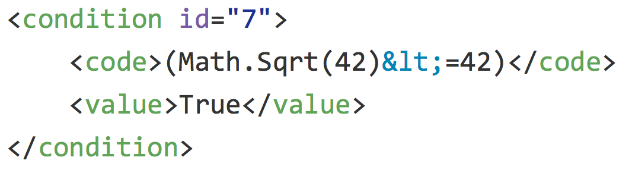
\includegraphics[width=2.4in]{fig_Complexity_file_test.png}
  \caption{Example test condition module.  Instantiated in
    Fig.~\ref{fig:example main file}, line 16.}
  \label{fig:example complexity-test file}
\end{figure}


\subsubsection{Code Complexity Modules}
\label{sec: complexity modules}

\begin{verbatim}
<complexity id="" type="" group="" executed="" in_out_var="i" 
                       need_condition="" indirection="" need_id="">
    <code></code>
    <body></body>
</complexity>
\end{verbatim}

\begin{itemize}
    \item id: string indicating this complexity.  Appears in the test case
      file name.  Typically this is a number.

    \item type: Used types are: \verb|if|, \verb|switch|, \verb|goto|,
    \verb|for|, \verb|foreach|, \verb|while|,
    \verb|function|, and \verb|class|.
    If the type is \verb|class|, source code in the \verb|<body></body>| is placed in
    an additional file that is created for this case.
    Invocation statements are generated for \verb|function| and \verb|class| types.

    An extra variable is created for \verb|foreach| type complexities (with group
    \verb|loops|).
    No other type has any effect on VTSG.

    \item group: Used groups are: \verb|conditionals|, \verb|jumps|,
    \verb|loops|, \verb|functions|, and \verb|classes|.
    No group, other than \verb|loops|, has any effect on VTSG.

    \item executed: whether the placeholder will be executed or not. Four 
    values are allowed:
    \begin{itemize}[nosep]
        \item 0: Never executed
        \item 1: Always executed
        \item condition:  Executed if the condition is true
        \item not\_condition:  Executed if the condition is false
    \end{itemize}
    Table~\ref{tab:execution examples} gives example code for each value.

    \item in\_out\_var: whether the variable (from the Input) will be used or
    transformed in the Complexity before being used in the Filter.  If the
    variable is neither used nor transformed, do not use this attribute.
    Three values are allowed:
    \begin{itemize}[nosep]
        \item in: the variable is used before the placeholder
        \item out: the variable is used after the placeholder
        \item traversal: the variable is used in the placeholder
    \end{itemize}
    If this attribute is used, the code should contain the following
    placeholders: \\
    \verb|{{in_var_name}}|, \verb|{{out_var_name}}|, and \verb|{{var_type}}|.

    \item need\_condition: ``1'' if this complexity needs a condition.
      This complexity is also combined with conditions (see
      Sec.~\ref{sec: condition modules}) if \verb|executed| is \verb|condition|
      or \\ \verb|not_condition|. (optional)

    \item indirection: ``1'' if the code is split into two chunks (call and
    declaration) or calls a function.  The body tag should be present when
    calling a function.

    \begin{table}[H]
    \centering
    \caption{An example of code for each value of ``executed'' showing whether
      ``placeholder'' code will be executed.}
    \begin{tabular}{|r|c|l|}
    \hline
      \makecell{Value of \\ ``executed''} &
      \makecell{When \\ executed} &
      example code \\
    \hline
    0 &
    never &
    \begin{minipage}{3in}
    \begin{verbatim}


    switch(6) {
      case(6):
        break;
      default:
        {{ placeholder }}
        break;
    }
    \end{verbatim}
    \end{minipage}
    \\
    \hline
    1 &
    always &
    \begin{minipage}{3in}
    \begin{verbatim}


    switch(6) {
      case(6):
        {{ placeholder }}
        break;
      default:
        break;
    }
    \end{verbatim}
    \end{minipage}
    \\
    \hline
    condition &
    \makecell{when \\ condition \\ is true} &
    \begin{minipage}{3in}
    \begin{verbatim}


    if ({{ condition }}) {
          {{ placeholder }}
    } else {
          {}
    }
    \end{verbatim}
    \end{minipage}
    \\
    \hline
    not\_condition &
    \makecell{when \\ condition \\ is false} &
    \begin{minipage}{3in}
    \begin{verbatim}


    if ({{ condition }}) {
          {}
    } else {
          {{ placeholder }}
    }
    \end{verbatim}
    \end{minipage}
    \\
    \hline
    \end{tabular}
    \label{tab:execution examples}
    \end{table}

    \item need\_id: ``1'' if the code has a placeholder, \verb|{{id}}|,
    to generate a unique ID for the Complexity.  This ID to generate 
    a label, a parameter, or a function name in a nested
    context.

    \item code: the source code of the Complexity.  Code or 
    body should contain \\ \verb|{{placeholder}}|
    where the Filter is inserted.  It may also contain
    \verb|{{condition}}| where the Condition
    is inserted.

    \item body: additional source code not in the main execution flow,
    e.g., functions or classes.  This code is placed in a separate file
    if the type is \verb|class|. (optional)
\end{itemize}


\begin{figure}[htbp]
  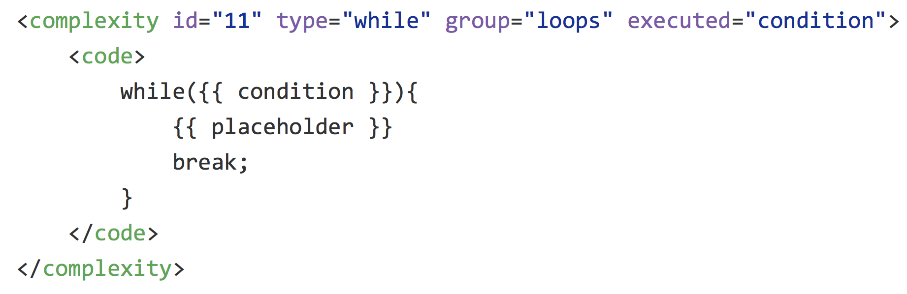
\includegraphics[width=4in]{fig_Complexity_file_while.png}
  \caption{Example Complexity module with a {\texttt while} loop.  Instantiated in 
    Fig.~\ref{fig:example main file}, lines 16--21.}
  \label{fig:example complexity-while file}
\end{figure}

\begin{figure}[htbp]
  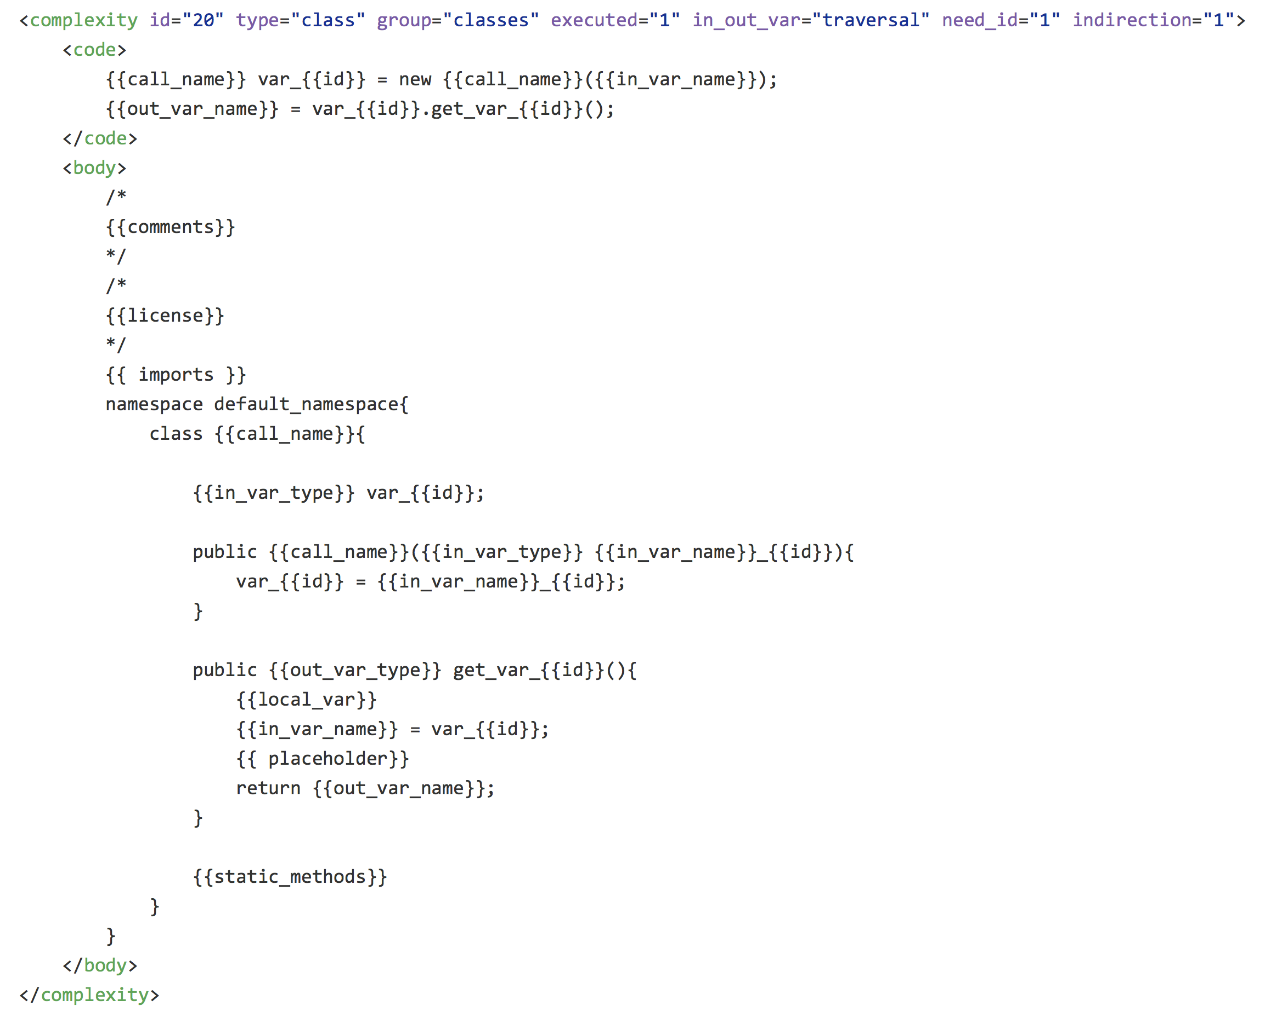
\includegraphics[width=\linewidth]{fig_Complexity_file_method.png}
  \caption{Example Complexity module with a method invocation.  
  The \texlangle code\texrangle\  part is instantiated in
  Fig.~\ref{fig:example main file}, lines 18 and 19. 
  The \texlangle body\texrangle\  part is instantiated in
  Fig.~\ref{fig:example aux file}.}
  \label{fig:example complexity-method file}
\end{figure}

VTSG can put several complexities in one test case.
The example in Sec.~\ref{sec:case file name} has two types of
Complexity: a control flow complexity and a data flow complexity. 
The control flow complexity specification is in 
Fig.~\ref{fig:example complexity-while file}.  It is instantiated in 
lines 16--21 of
Fig.~\ref{fig:example main file}.  Line 16 is the instantiation of 
the control flow condition
specified in Fig.~\ref{fig:example complexity-test file}.

The data flow complexity is a method call within the \verb|while| loop.  
The specification
is in Fig.~\ref{fig:example complexity-method file}.  
The \verb|<code>|
part is instantiated in lines 18 and 19 of 
Fig.~\ref{fig:example main file}. 
The \verb|<body>| part is instantiated in
Fig.~\ref{fig:example aux file}.


\section{Adding to VTSG}

The next subsection is a brief tutorial giving suggestions on how to add a new
flaw to an existing language in VTSG.  The subsection after that has suggestions
on how to add a new language.  The final subsection offers some guidance on
adding new capabilities or features to VTSG itself.

\subsection{How to Add a Flaw}

The easiest way to add a new flaw is modify a similar existing flaw to present the
new flaw.  If nothing is suitable, here is a tutorial for writing a brand new flaw.

There are so many interacting specifications for a flaw, it is best to write it in
three steps: first, write an example of the flaw in regular source code; second,
decide how to
divide the code among modules, and third, specify the pieces in VTSG.

\subsubsection{Write an Example With the Flaw}

As a first step, choose a generated test case and modify the source code to present
the target flaw.  Here is the core code of
a potential divide by zero guarded by a filter:
\begin{verbatim}
    if data == 0:
        print('Invalid input')
        sys.exit(1)

    print(f'The reciprocal of {data} is {1/data}')
\end{verbatim}
You may want to try different variants to find which fits your needs best.  For
instance, one variant of this flaw is for the filter to provide a safe value instead
of aborting, like this:
\begin{verbatim}
    if data == 0:
        print('Invalid input')
        data = 1

    print(f'The reciprocal of {data} is {1/data}')
\end{verbatim}
Another variant is for the weakness itself to be guarded by the filter:
\begin{verbatim}
    if data != 0:
        print(f'The reciprocal of {data} is {1/data}')
    else:
        print('Invalid input')
\end{verbatim}

It helps later checking to write the code to demonstrate the failure, instead of
failing silently.  In the above code if division by zero is ever attempted, Python
aborts with failure messages.  In contrast consider a path traversal weakness.  Path
traversal is when the user might access private directories.  Here is a simple
version.  It intends to open a file named by the user in the \verb|/home| directory:
\begin{verbatim}
    tainted_1 = input() # read one line

    file = os.path.join('/home', tainted_1)
    f = open(file, 'r')
\end{verbatim}
Running this with an input that exploits the weakness, like
\verb|../etc/passwd|, doesn't give any indication that the exploit succeeded.  The
file is opened and then the program ends.  The following variant is better.  It
prints a line from the password file to demonstrate the exploit:
\begin{verbatim}
    tainted_1 = input() # read one line

    file = os.path.join('/home', tainted_1)
    with open(file, 'r') as f:
        print(f.readline(), end='')
\end{verbatim}


\subsubsection{Decide What is Input, What is Filter, What is Sink, etc.}

The second step is to decide what parts of the code are inputs, what parts are
filters (which will be wrapped in complexities), and what parts are sinks.

If you want to generate cases where some piece of code may or may not be executed,
put that code in Filter modules.  The second example above might generate a case
like this.  (Comments show the origin of each piece of source code.)
\begin{verbatim}
    # Complexity
    if True:
        # Filter
        if data == 0:
            print('Invalid input')
            data = 1

    # Sink
    print(f'The reciprocal of {data} is {1/data}')
\end{verbatim}

If the sink is guarded, as in the third example, it may need to be a Filter module.
In this case, the ``Sink'' module may be empty.
\begin{verbatim}
    # Complexity
    if True:
        # Filter
        if data != 0:
            print(f'The reciprocal of {data} is {1/data}')
        else:
            print('Invalid input')
\end{verbatim}


\subsubsection{Write the Modules}

Now that you have an idea of how to split up the code, the third step is to
write new modules for VTSG for the flaw.  You probably need to write new sinks
and filters, but you should be able to use existing input and exec query
modules.  Edit the sinks.xml (or filters.xml or other) file to add them,
then run VTSG.  It's likely that nothing is generated the very first time you
try because VTSG cannot find an input and filter compatible with your new sink.

\label{sec:connecting inputs, filters, and sinks}
Figure~\ref{fig:VTS operation overview} suggests that the result of the Input module
connects to and must match the input of the Filter module, and its output connects to
and must match the input of the Sink.  These modules are shown together in
Fig.~\ref{fig:input, filter, and sink}.
\begin{figure}[htbp]
  \centerline{
\includegraphics[width=\linewidth]{fig_input_filter_sink.png}}
  \caption{The result of the Input module connects to the input of the Filter module,
    its output connects to the input of the Sink module, and its output connects
    to the input of the Exec Query module.
  }
  \label{fig:input, filter, and sink}
\end{figure}
Compatibility of inputs, filters, sinks, and exec queries is computed various
ways.  Remember that
VTSG first chooses a sink module then chooses compatible filter, input, and exec
query modules to
use with it.
\label{sec:compatible modules}
A filter is used with a sink if
\begin{enumerate}[nosep]
\item the filter \verb|output_type| is ``nofilter'' or the same as the sink
  \verb|input_type| \emph{and}
\item the filter has a \verb|flaw_type| that is ``default'' or is the same as the
  sink \verb|flaw_type|.
\end{enumerate}
Figure~\ref{fig:how filters fit a sink} suggests that filters A, B, and C will
be used with the sink.
\begin{figure}[htbp]
  \centerline{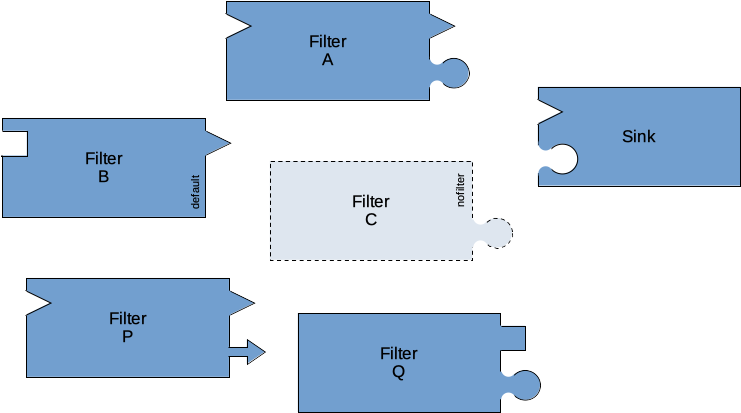
\includegraphics[width=.8\linewidth]{fig_filters_and_sinks.png}}
  \caption{How filters are chosen for a sink.  Filters A, B, and C will be used.
    Filter P is not used because the flaw\_type differs.
    Filter Q is not used because the output\_type differs.
  }
  \label{fig:how filters fit a sink}
\end{figure}
Filter B is compatible because the \verb|flaw_type| is
``default''; it is compatible with any type of flaw.  Filter C is ``nofilter'' and
just passes the value through.  Filter P is never used with that sink because
the \verb|flaw_type| is not the same.
Filter Q is never used because the \verb|output_type| is not the same as the
sink \verb|input_type|.

An input is used with a sink and a filter if
\begin{enumerate}[nosep]
\item the filter \verb|input_type| is ``nofilter'' and the \verb|output_type|
  of the input is the same as the sink \verb|input_type| \emph{or}
\item the filter \verb|input_type| is something other than ``nofilter'' and the
  \verb|output_type| of the input is the same as the filter \verb|input_type|.
\end{enumerate}
Fig.~\ref{fig:how inputs fit} illustrates this matching rule.  Input 1 is used with
Filter A, and Input 2 is used with Filter B.  Input 1 is also used with Filter C
because Filter C is ``nofilter'' and Input 1 matches the sink.
\begin{figure}[htbp]
  \centerline{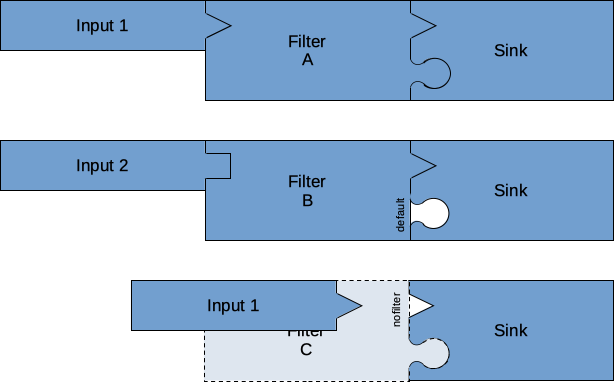
\includegraphics[width=.667\linewidth]{fig_inputs_filters_and_sinks.png}}
  \caption{How inputs are chosen for a filter and sink.  Input 1 is used with
    Filter A.  Input 2 is used with Filter B.  Input 1 is also used with Filter C
    because Filter C is ``nofilter'' and Input 1 matches the sink.
  }
  \label{fig:how inputs fit}
\end{figure}

Be aware that \emph{any} string may be in the \verb|input_type| or
\verb|output_type|.
This allows you to use a kind of ``extended types'' to connect specific inputs,
filters, and sinks.  Following is an example is in Python.
I wanted the input to be wrapped in
complexities, like the following:
\begin{verbatim}
    # Input
    tainted_1 = None

    # Complexity
    if 5 == 5:
        # Filter
        tainted_1 = input()

    # Sink
    if tainted_1 is not None:
        # flaw # no validation - allows arbitrary execution
        sys.path += [tainted_1]
        print(f'added { tainted_1 } to Python module search path')
\end{verbatim}
Variables aren't declared in Python, but I had to initialize the variable to
\verb|None| in case the input is not executed.  I declared the variable in the input
module and put the input code in the filter module, so that the input code would be
wrapped in complexities.  I used custom types \verb|string,filter_input| to connect
the sink to the ``filter'' (really, input) and \verb|InitToNone| to connect the
``filter'' to the ``input'' (really, initialization).

\subsubsection{Making Sure Case Safety is Computed Correctly}

Figuring out how to mark the modules as safe or unsafe can be tricky.
The following code may allow a large \emph{negative} index access, and thus cause an
exception.  I thought this is always unsafe.
\begin{verbatim}
    if index < len(array):
        print(array[index])
\end{verbatim}
I discovered my mistake when I executed the cases and ``unsafe'' cases did
\emph{not} produce any evidence of a successful exploit.  I realized that, if the
``input'' was a safe hardcoded
value, the code was safe!
\begin{verbatim}
    index = 0

    if index < len(array):
        print(array[index])
\end{verbatim}
The proper marking is that the sink is neither always safe nor always unsafe.
A proper filter or guard can make it safe.
See Sec.~\ref{sec:safe or unsafe} for details.


\subsection{How to Add a Language}
\label{sec:add a language}

The easiest way is to
\begin{enumerate}[nosep]
\item decide the short name of the language, e.g., py for Python or php for
  PHP.  Using the extension of those programs is a good idea.
\item create a directory by that name under src/template
\item copy the six files of an existing language
\item change the name attribute in file\_template.xml to the language name.
\end{enumerate}
Change language characteristics in all the files.  Generate a few cases and
execute them to make sure syntax and other details are correct.  It's best to
start by converting just one or two sinks, inputs, and filters for quick turn around.
Comment out all the rest of the modules to start.
As you convert or add flaws, you may find that some language specifications need
adjustment.


\subsection{Adding New Capabilities to VTSG}

New VTSG capabilities often allow the user who is describing programming languages or
flaws to make new mistakes.  Suppose input modules now have a \verb|parallel|
attribute, which must have one or more types of processing, such as Single
Instruction, Single Data (SISD); Multiple Instruction, Single Data (MISD); Single
Instruction, Multiple Data (SIMD); Multiple Instruction, Multiple Data (MIMD); Single
Program, Multiple Data (SPMD), or Massively Parallel Processing (MPP).  What should
VTSG do when the user gives an input module a \verb|parallel| attribute, but no type
of processing?  VTSG code could just crash with a traceback about \verb|NoneType|
object.  This does not help the user much.

If the user can make a mistake, such as mismatched attributes or invalid fields, VTSG
should explain what the problem is, where it arose, why it is invalid (e.g. where the
information will be used), and what are the correct approaches or alternatives.  For
example, for an empty \verb|<dir></dir>| in an input module, VTSG reports
\begin{verbatim}
[ERROR] Invalid empty <dir></dir> in the inputs file.
A dir string is required; it is used in the name of the generated file.
\end{verbatim}
then exits.

In case of an error due to a bug in VTSG itself, it may crash.  In theory, VTSG
developers will find and fix all bugs before the user runs it.


\section{Generated Test Case File Names}

This section describes how the names of test case files are created.

VTSG creates directories and subdirectories for the test cases that it generates.
The directory structure is described in
Sec.~\ref{sec:case directory structure}.

%\subsection{Test Case File Names}
\label{sec:case file name}

VTSG names test case files as
\verb|FLAW__I_INPUT__F_FILTER__S_SINK__EQ_EXEC_| \\
\verb|QUERY__NMBCPLX-CMPLX1[.COND]-CMPLX2[.COND]x.EXT|
\begin{itemize}[nosep]
    \item FLAW: Flaw type, e.g. CWE\_89, BF, or STR30-PL, see
	Sec.~\ref{sec:sink modules}.
    \item INPUT: Input description (dirs), see Sec.~\ref{sec:module description} (optional)
    \item FILTER:  Filter description (dirs) (optional)
    \item SINK:  Description (dirs) of the critical function
    \item EXEC\_QUERY:  ExecQuery description (dirs) (optional)

    \item NMBCPLX:  The number of complexities.
    \item CMPLX1[.COND], CMPLX2[.COND], \ldots: List of complexities.
            CMPLX is the id in the code complexity module,
            see Sec.~\ref{sec: complexity modules}.
            If the complexity has a
            condition, COND is the id in the test condition module,
            see Sec.~\ref{sec: condition modules}.
            Tables \ref{tab:complexity IDs for CSharp},
            \ref{tab:complexity IDs for PHP}, and
            \ref{tab:complexity IDs for Python} in the language appendixes list
            complexity ids defined in \CSharp, PHP, and Python.
            Tables \ref{tab:condition IDs for CSharp},
            \ref{tab:condition IDs for PHP}, and
            \ref{tab:condition IDs for Python} list condition
            ids defined in \CSharp, PHP, and Python. (optional)
    \item x: Sequence of the file within the test.  If the test consists of just one
      file, there is no sequence letter.  If the test consists of more than one file,
      that is, when the complexity \verb|type| is \verb|class|,
      see Sec.~\ref{sec: complexity modules},
      the main file is ``a'', and other files, such as classes, are ``b'', ``c'',
      ``d'', etc. (optional)
    \item EXT: file extension, given in the \verb|file_template.xml| file, see
    Sec.~\ref{sec: file template}.
\end{itemize}

File names reflect the entire case, not just the code in a
particular file.  If a case consists of more than one file, as in the
example used in this manual, all files have
identical names, except for the final sequence letter.

\begin{figure}[htbp]
  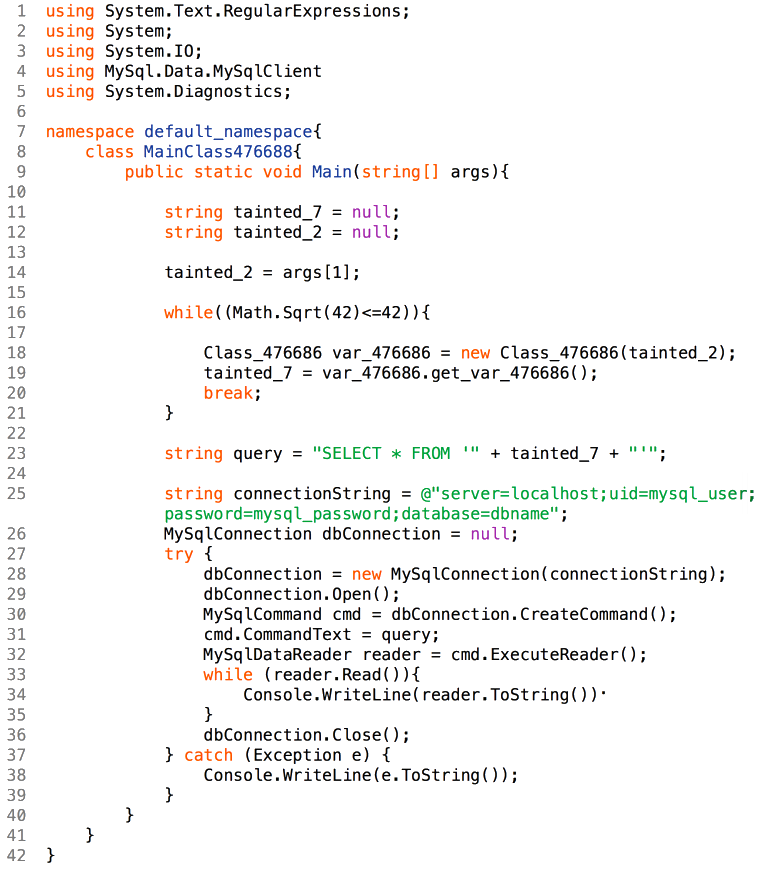
\includegraphics[width=\linewidth]{fig_example_code1.png}
  \caption{Main file of example. Line 14 instantiates input code from 
    Fig.~\ref{fig:example input file}. Lines 16--19 instantiates complexity code from 
    Fig.~\ref{fig:example complexity-while file}. Line 16 instantiates condition code from
    Fig.~\ref{fig:example complexity-test file}.  Lines 18 and 19 instantiate code from the
    \texlangle code\texrangle\  part of Fig.~\ref{fig:example complexity-method file}.
    Line 23 instantiates critical preparation code from Fig.~\ref{fig:example sink file}.
    Lines 25--39 instantiate query execution code from Fig.~\ref{fig:example exec-query file}.
  }
  \label{fig:example main file}
\end{figure}

\begin{figure}[htbp]
  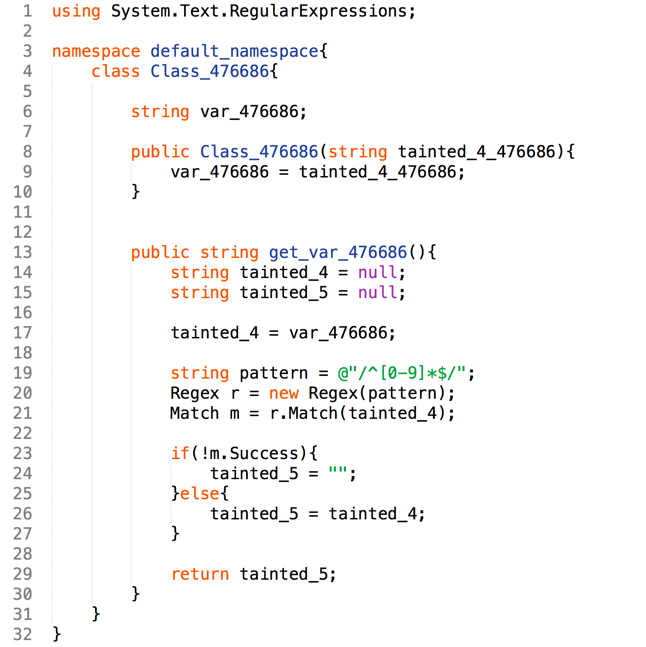
\includegraphics[width=0.85\linewidth]{fig_example_code2.png}
  \caption{Auxiliary file of example.  It instantiates code from the
    \texlangle body\texrangle\ part of Fig.~\ref{fig:example complexity-method file}.
    Lines 19--27 instantiate filter code
    from Fig.~\ref{fig:example filter file}.}
  \label{fig:example aux file}
\end{figure}

As an example of a file name, consider the test case used in this manual.  The case
consists of
two files.
Fig.~\ref{fig:example main file} is the main file of the example.  
Fig.~\ref{fig:example aux file} is an auxiliary class file.  
The code in
the main file invokes the class at line 18.

The name of the main file is
\verb|CWE_89__I_shell_commands__F_func_preg_match-| \\
\verb|only_numbers__S_select_from-concatenation_simple_quote__sql_server| \\
\verb|__2-11.7-20a.cs|.
The name of the class file, Fig.~\ref{fig:example aux file}, is
identical, except for the
file letter ``b'' instead of ``a'' at the end.

The extension, cs, shows that it is a \CSharp\ file.
We understand the file name as follows:

\noindent CWE 89: Improper Neutralization of Special Elements used in an SQL Command
('SQL Injection') \cite{CWE89}

\noindent The input comes from shell\_commands, see specification in
Fig.~\ref{fig:example input file}.

\noindent The filter is func\_preg\_match-only\_numbers,
Fig.~\ref{fig:example filter file}.

\noindent The sink is select\_from-concatenation\_simple\_quote\_\_sql\_server,
Fig.~\ref{fig:example sink file}.

\noindent The last part, 2-11.7-20, describes the complexities.
The first number, 2, means this has two complexities.
Tables~\ref{tab:complexity IDs for CSharp} and
\ref{tab:condition IDs for CSharp} help us decode them.
The first, outer complexity is 11 with condition 7. 11 is \verb|while|,
Fig.~\ref{fig:example complexity-while file}, 
with condition 7 meaning \verb|Math.Sqrt(42)<=42|, which always evaluates to true,
Fig.~\ref{fig:example complexity-test file}.
The second, inner complexity is 20 meaning the sink code is executed in the class body,
Fig.~\ref{fig:example complexity-method file}.

\noindent ``a'' means this is the main file.



\section{Acknowledgments}

Bertrand Stivalet and Aurelien Delaitre, from the NIST SAMATE team, designed the
architecture of the VTSG and managed its implementation.  The project was
implemented by students from TELECOM Nancy: Jean-Philippe Eisenbarth, Valentin
Giannini, and Vincent Noyalet.  We thank Terry Cohen for her comments and
suggestions, which improved this report.  We also thank Elizabeth Fong and
Charles de Oliveira for their contributions to this report.
% On 12 June 2020, Terry Cohen wrote the following [[much editing by PEB]]
% Bertrand and Liz wrote the original document. I did some quick grammatical editing. Liz submitted it, but Barbara wanted it to cover both C# and PHP. The original did not have both. Because of the SATE V and CSIAC projects, this was put on hold.
%
% As I revised the NIST IR, I went through all of the instructions to verify the PHP statistics in the paper that Bertrand and Liz published and to generate C# statistics. I discovered errors and/or missing commands in the instructions. Charles pointed out the missing instructions.
%
% I recommend crediting Bertrand and Liz, because they started documentation.  I
% wrote the new document covering both C# and PHP.
%
% I added Charles because he helped me find the missing commands.  At the time, he was indifferent to being listed as a co-author.  We were using it as a learning exercise.
%
% In summary, I recommend that Bertrand, Liz, you, and your team be listed as co-authors.


% references section
\addcontentsline{toc}{section}{References}
\bibliographystyle{techpubs}
\bibliography{vulTestSuiteGenV3}

\newpage

%%%%%%%%%%%%%%%%%%%%%%%%%%%%%%%%%%%%%%%%%%%%%%%%%%%%%%%%%%%%%%%%%%%%%
%
%           APPENDIX
%
%%%%%%%%%%%%%%%%%%%%%%%%%%%%%%%%%%%%%%%%%%%%%%%%%%%%%%%%%%%%%%%%%%%%%

% make the Appendix begin on a new page (not a new column) even in
% two-column mode
\clearpage

\appendix

\section{\CSharp\ Language}
\label{sec:CSharp language}

This appendix documents the flaws, flaw groups, complexities, and conditions
currently in the
\CSharp\ language files.
It also gives instructions how to compile and run the test cases.

The following flaws are currently defined for this language:
\begin{itemize}[nosep]
    \item SQL Injection (CWE-89)
    \item XPath Injection (CWE-91)
    \item LDAP Injection (CWE-90)
    \item OS Command Injection (CWE-78)
    \item Path traversal (CWE-22)
    \item Information Leak Through Error Message (CWE-209)
    \item Storing Password in Plain Text (CWE-256)
    \item Use of Insecure Cryptographic Algorithm (CWE-327)
    \item NULL Pointer Dereference (CWE-476)
\end{itemize}

\vspace{1em}

The flaws are in the following groups:
\begin{itemize}[nosep]
    \item OWASP\_a1 has CWE\_78, CWE\_89, CWE\_89, CWE\_89, CWE\_90, CWE\_91,
      CWE\_91, and CWE\_91.
    \item OWASP\_a2 has CWE\_256.
    \item OWASP\_a4 has CWE\_22.
    \item OWASP\_a5 has CWE\_209.
    \item OWASP\_a6 has CWE\_327
    \item OWASP\_a9 has CWE\_476.
\end{itemize}

\newpage

Here are the complexities currently available in \CSharp.
We explain the concept of code complexities in Sec.~\ref{sec:code complexities} and
the format of complexity modules in Sec.~\ref{sec: complexity modules}.
The brief descriptive pseudocode reminds the reader of the complexity.
See the \verb|complexity.xml| file for the specific code.

\begin{table}[H]
\centering
\caption{Complexity IDs and pseudocode defined for \CSharp}
\begin{tabular}{|r|l|}
\hline
\textbf{ID} & \textbf{Pseudocode} \\
\hline
 1 & if condition code \\
\hline
 2 & if condition code else \\
\hline
 3 & if condition else code \\
\hline
 4 & if condition code else if not condition \\
\hline
 5 & if condition else if not condition code \\
\hline
 6 & if condition code else if not condition else \\
\hline
 7 & if condition else if not condition code else \\
 \hline
 8 & if condition else if not condition else code \\
\hline
 9 & switch code executed \\
\hline
10 & switch code not executed \\
\hline
11 & while code \\
\hline

12 & do code while \\
\hline
13 & for code \\
\hline
14 & foreach code \\
\hline
15 & goto code not executed \\
\hline
16 & goto code executed \\
\hline
17 & function body executes code \\
\hline
18 & input passed via function then code \\
\hline
19 & code then output passed via function \\
\hline
20 & class body executes code \\
\hline
21 & input passed via class then code \\
\hline
22 & code then output passed via class \\
\hline
\end{tabular}
\label{tab:complexity IDs for CSharp}
\end{table}

\newpage

Here are the conditions currently available to be used in code complexities.
We explain condition modules in Sec.~\ref{sec: condition modules}.
Table~\ref{tab:condition IDs for CSharp} shows the ID, the code, and whether it
always evaluates to true or false.

\begin{table}[H]
\centering
\caption{Condition IDs, code, and value to which it evaluates defined for
  \CSharp}
\begin{tabular}{|r|l|l|}
\hline
\textbf{ID} & \textbf{Code} & \textbf{Value} \\
\hline
1 & \verb|1==1| & True \\
\hline
2 & \verb|1==0| & False \\
\hline
3 & \verb|4+2<=42| & True \\
\hline
4 & \verb|4+2>=42| & False \\
\hline
5 & \verb|Math.Pow(4, 2)<=42| & True \\
\hline
6 & \verb|Math.Pow(4, 2)>=42| & False \\
\hline
7 & \verb|Math.Sqrt(42)<=42| & True \\
\hline
8 & \verb|Math.Sqrt(42)>=42| & False \\
\hline
\end{tabular}
\label{tab:condition IDs for CSharp}
\end{table}


\label{sec:run csharp}
To compile and run \CSharp\ test cases, install \emph{mono} and \emph{mcs}.
The Mono project created \emph{mono} as an open source platform that
implements the .NET Framework. Class libraries and \CSharp\ compilation are enabled
by \emph{mcs}. See \href{http://github.com/mono/mono}{http://github.com/mono/mono}.

Here is the command to install mono:

\begin{verbatim}
    sudo apt-get install mono-complete
\end{verbatim}

Here is the command to install mcs:

\begin{verbatim}
    sudo apt-get install mcs
\end{verbatim}

On a Mac, install Homebrew first. See
\href{https://brew.sh/}{https://brew.sh/}.
Then use homebrew to install mono.  See \href{https://formulae.brew.sh/formula/mono}{https://formulae.brew.sh/formula/mono}.

The script \verb|compilationTester.sh| uses mcs to compile all the
\CSharp\ cases that are generated.

\section{PHP Language}
\label{sec:PHP language}

This documents the flaw, flaw group, complexities, and conditions currently in the
PHP language files.

The following flaw is currently defined for this language.  The flaw group is in
parentheses.
\begin{itemize}
    \item SQL Injection (CWE-89) (OWASP\_injection)
\end{itemize}

\newpage

Here are the complexities currently available in PHP.
We explain the concept of code complexities in Sec.~\ref{sec:code complexities} and
the format of complexity modules in Sec.~\ref{sec: complexity modules}.
The brief descriptive pseudocode reminds the reader of the complexity.
See the \verb|complexity.xml| file for the specific code.

\begin{table}[H]
\centering
\caption{Complexity IDs and pseudocode defined for PHP}
\begin{tabular}{|r|l|}
\hline
\textbf{ID} & \textbf{Pseudocode} \\
\hline
 1 & if condition code \\
\hline
 2 & if condition code else \\
\hline
 3 & if condition else code \\
\hline
 4 & if condition code else if not condition \\
\hline
 5 & if condition else if not condition code \\
\hline
 6 & if condition code else if not condition else \\
\hline
 7 & if condition else if not condition code else \\
 \hline
 8 & if condition else if not condition else code \\
\hline
 9 & switch code executed \\
\hline
10 & switch code not executed \\
\hline
11 & while code \\
\hline

12 & do code while \\
\hline
13 & for code \\
\hline
14 & foreach code \\
\hline
15 & goto code not executed \\
\hline
16 & goto code executed \\
\hline
17 & function body executes code \\
\hline
18 & input passed via function then code \\
\hline
19 & code then output passed via function \\
\hline
20 & class body executes code \\
\hline
21 & input passed via class then code \\
\hline
22 & code then output passed via class \\
\hline
\end{tabular}
\label{tab:complexity IDs for PHP}
\end{table}


Here are the conditions currently available to be used in code complexities.
We explain condition modules in Sec.~\ref{sec: condition modules}.
Table~\ref{tab:condition IDs for PHP} shows the ID, the code, and whether it
always evaluates to true or false.

\begin{table}[H]
\centering
\caption{Condition IDs, code, and value to which it evaluates defined for
  PHP}
\begin{tabular}{|r|l|l|}
\hline
\textbf{ID} & \textbf{Code} & \textbf{Value} \\
\hline
1 & \verb|1==1| & True \\
\hline
2 & \verb|1==0| & False \\
\hline
\end{tabular}
\label{tab:condition IDs for PHP}
\end{table}


\section{Python Language}
\label{sec:Python language}

This documents the flaws, flaw groups, complexities, and conditions currently in the
Python language files.

The following flaws are currently defined for Python.  The flaw group is in
parentheses.  Flaws in the ``Exception'' flaw group are caught by the Python runtime.
These are unlikely to be vulnerabilities (except denial of service).
\begin{itemize}[nosep]
    \item OS Command Injection (CWE-78) (OWASP\_a1)
    \item SQL Injection (CWE-89) (OWASP\_a1)
    \item Path traversal (CWE-22) (OWASP\_a4)
    \item Information Leak Through Error Message (CWE-209) (OWASP\_a5)
    \item Loop on Unchecked Input (CWE-606) (Other)
    \item Relative Path Traversal (CWE-23) (Other)
    \item Divide by Zero (CWE-369) (Exception)
\end{itemize}

\newpage

Here are the complexities currently defined.
We explain the concept of code complexities in Sec.~\ref{sec:code complexities} and
the format of complexity modules in Sec.~\ref{sec: complexity modules}.
The brief descriptive pseudocode reminds the reader of the complexity.
See the \verb|complexity.xml| file for the specific code.

\begin{table}[H]
\centering
\caption{Complexity IDs and pseudocode defined for Python}
\begin{tabular}{|r|l|}
\hline
\textbf{ID} & \textbf{Pseudocode} \\
\hline
 1 & if condition code \\
\hline
 2 & if condition code else \\
\hline
 3 & if condition else code \\
\hline
 4 & if condition code elif not condition \\
\hline
 5 & if condition elif not condition code \\
\hline
 6 & if condition code elif not condition else \\
\hline
 7 & if condition elif not condition code else \\
 \hline
 8 & if condition elif not condition else code \\
\hline

 11 & match case code not executed \\
\hline
 12 & match case code executed \\
\hline
 13 & no match case code executed \\
\hline
 14 & no match case code not executed \\
\hline

20 & while condition code break \\
\hline
20n & while condition break code \\
\hline
22 & for range(0, 1) code \\
\hline
22 & for array if value code \\
\hline

50 & function body executes code \\
\hline
51 & input passed via function then code \\
\hline
52 & code then output passed via function \\
\hline

70 & class body executes code \\
\hline
71 & input passed via class then code \\
\hline
72 & code then output passed via class \\
\hline
\end{tabular}
\label{tab:complexity IDs for Python}
\end{table}

\newpage

Here are the conditions currently available to be used in code complexities.
We explain condition modules in Sec.~\ref{sec: condition modules}.
This table shows the ID, the code, and whether it
always evaluates to true or false.

\begin{table}[H]
\centering
\caption{Condition IDs, code, and value to which it evaluates defined for
  Python}
\begin{tabular}{|r|l|l|}
\hline
\textbf{ID} & \textbf{Code} & \textbf{Value} \\
\hline
1 & \verb|1==1| & True \\
\hline
2 & \verb|1==0| & False \\
\hline
2u & True & True \\
\hline
2v & False & False \\
\hline
3 & \verb|4+2<=42| & True \\
\hline
3u & \verb|5==5| & True \\
\hline
3v & \verb|5!=5| & False \\
\hline
4 & \verb|4+2>=42| & False \\
\hline
5 & \verb|math.pow(4, 2)<=42| & True \\
\hline
6 & \verb|math.pow(4, 2)>=42| & False \\
\hline
7 & \verb|math.sqrt(42)<=42| & True \\
\hline
8 & \verb|math.sqrt(42)>=42| & False \\
\hline
\end{tabular}
\label{tab:condition IDs for Python}
\end{table}


% make this begin on a new page (not a new column) even in
% two-column mode
\clearpage

\section{Contents of git Repository}
\label{gitContent}

\begin{figure}[htbp]
  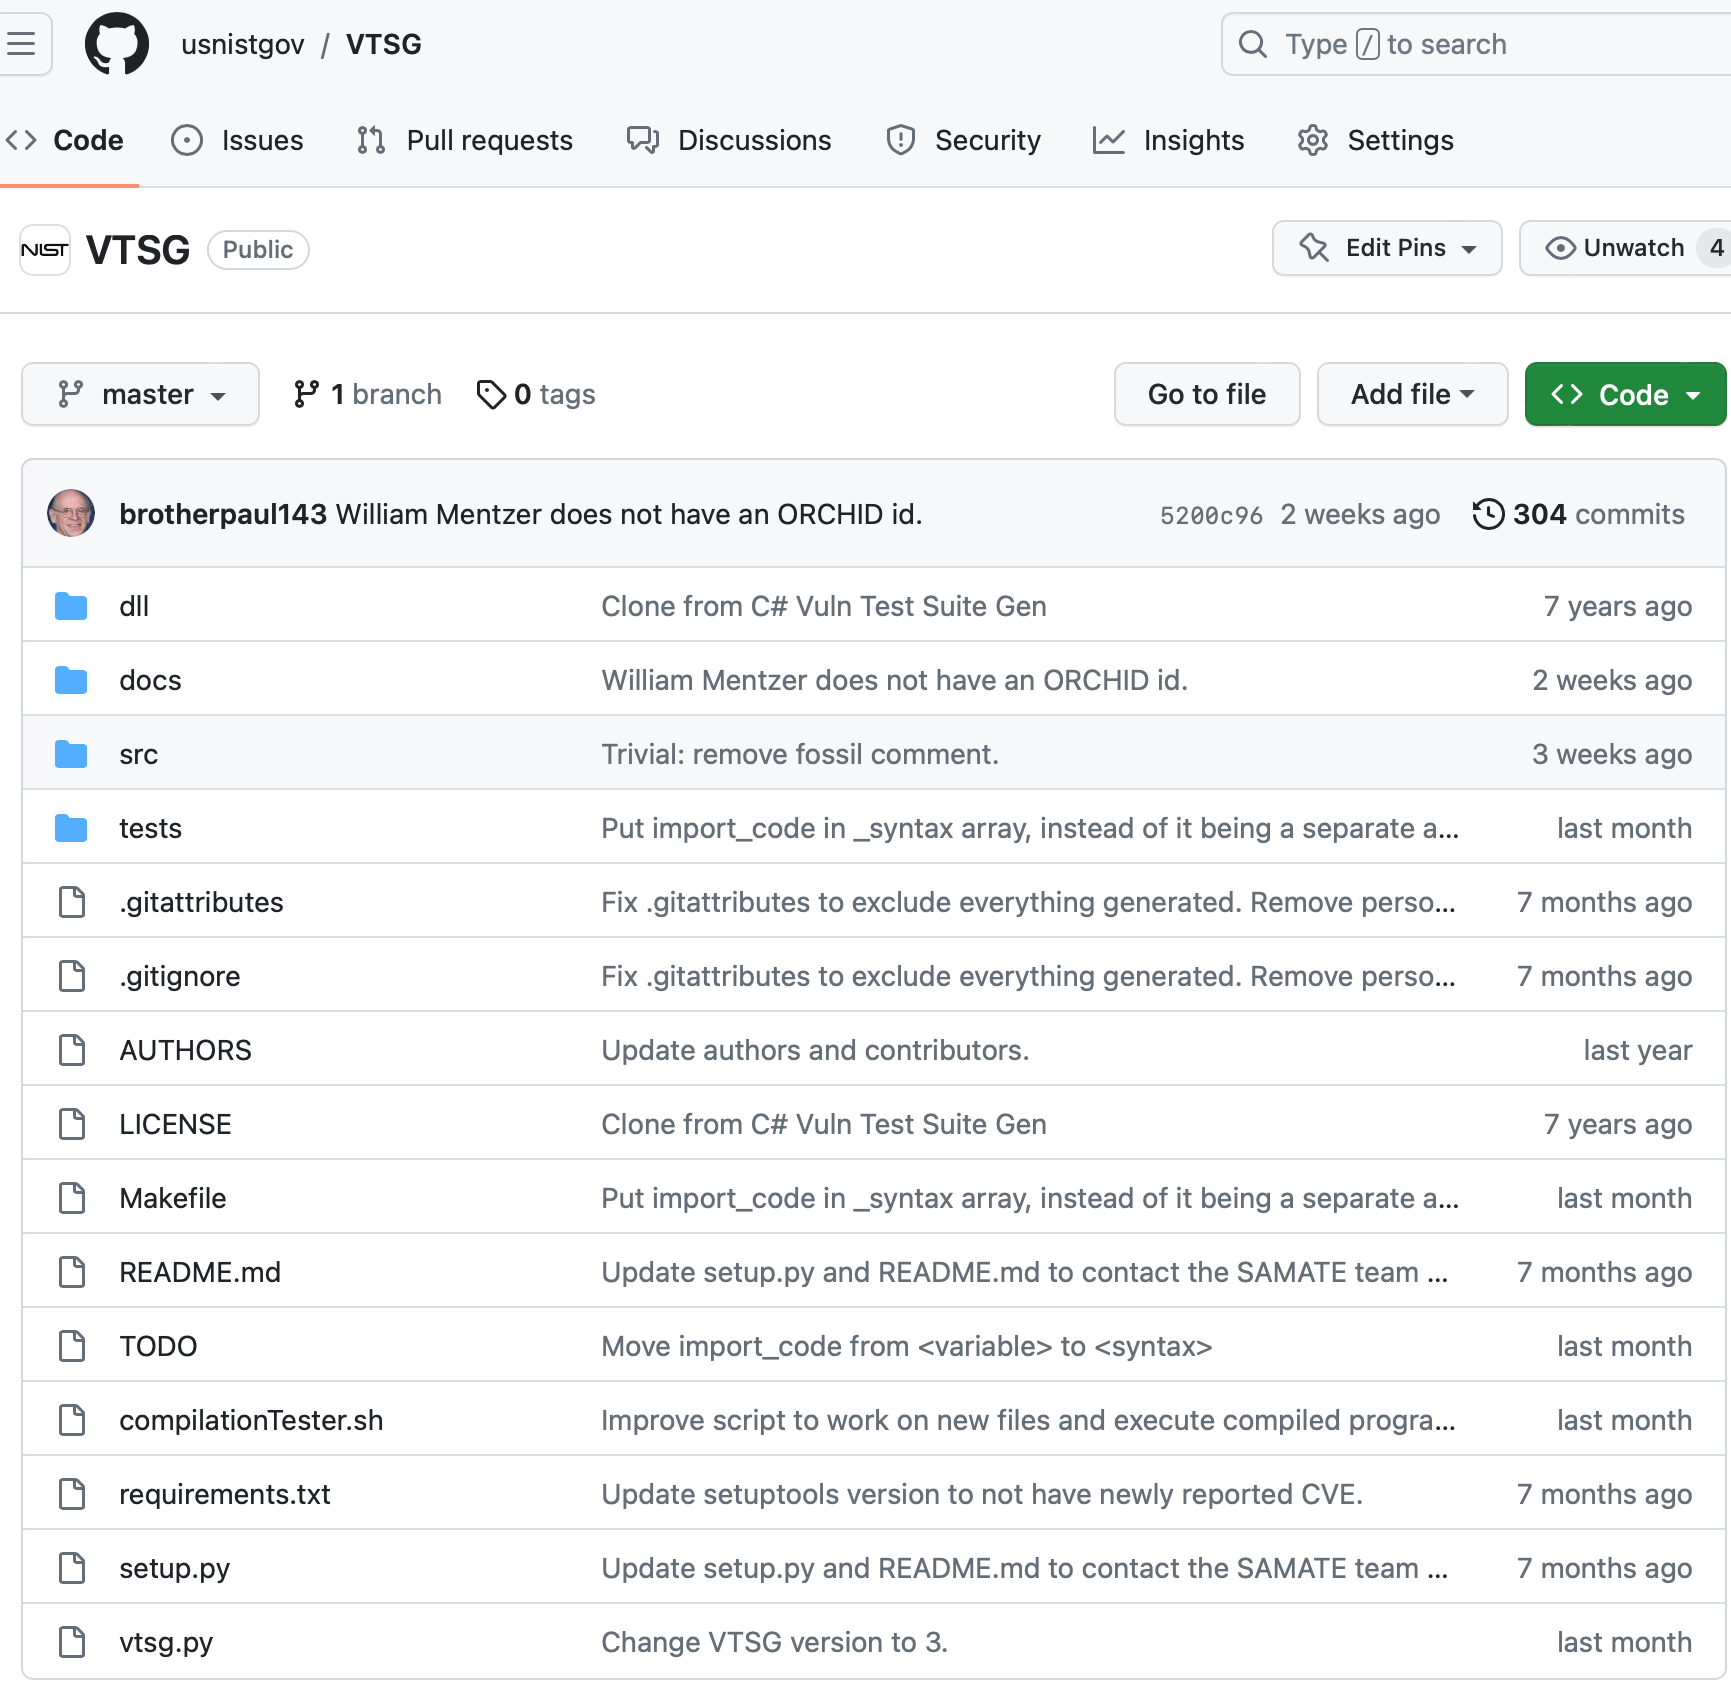
\includegraphics[width=1\linewidth]{fig_git_files.png}
  \caption{Snapshot of files in the VTSG git repository, which is at
    \href{https://github.com/usnistgov/VTSG}{https://github.com/ usnistgov/VTSG},
    as of 12 January 2023.}
  \label{fig:git files}
\end{figure}

\begin{figure}[htbp]
  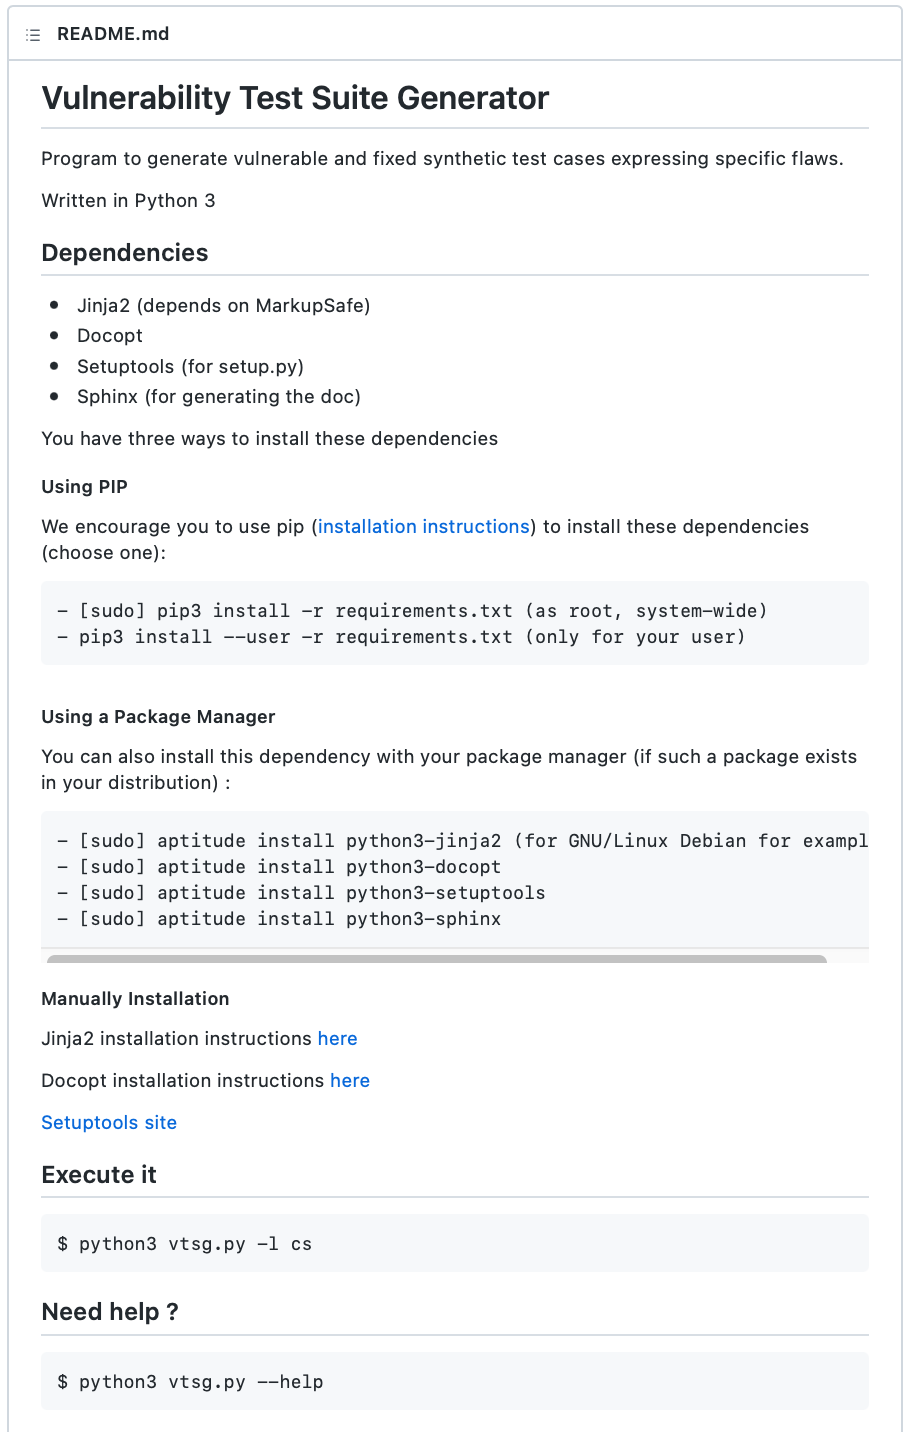
\includegraphics[width=0.8\linewidth]{fig_README_md.png}
  \caption{README.md file, which is at
    \href{https://github.com/usnistgov/VTSG/blob/master/README.md}
         {https://github.com/usnistgov/VTSG/blob/ master/README.md},
    as of 8 March 2022.}
  \label{fig:README.md file}
\end{figure}


%\section*{Appendix B: Change Log}
%\addcontentsline{toc}{section}{Appendix B: Change Log}
%If updating document with errata, detail changes made to document – delete if not applicable. \\

\end{document}
